\documentclass[../main.tex]{subfiles}
\begin{document}{}

In this section we will present our experimental results. We use two real world datasets, the first for modelling vehicle trajectory and the second for modelling UAV flight behavior.
We partition our datasets into in and out-of-distribution splits in order to evaluate the behavior of our models in the OOD case. We split our in-distribution data into train and test splits.  
In the next section we will explain our datasets, metrics, and baselines. 

\section{Setup}

We start this section by a quick recap of our model of uncertainties and some quick notation, then we will talk about our dataset and evaluation metrics in the following subsections, before we move on to the results.

Recall that we model two types of uncertainty. The aleatoric uncertainty, which is captured by the model output $\sigma_y$. Recall that for an input $x$, our model gives the predictive distribution $\pdf{y|x, \theta} = \mathcal{N}(\mu_y, \sigma_y)$. 
$\sigma_y$ is the std of a Gaussian which represents the model's belief about the true outcome $y$. The wider the Gaussian, the more uncertain the model is about $y$. We will use the shorthand $\mathcal{A}(x) = \sigma_y$, to directly talk about the model's aleatoric uncertainty for an input.

For the epistemic uncertainty, we will follow the same notation with $\mathcal{E}(x)$ is the model's epistemic uncertainty for point $x$. Recall that the epistemic uncertainty is the negative log probability our density model assigns to $x$ 
$$
    \mathcal{E}(x) = -log(\pdf{x|\theta}) 
    = -[log(\mathcal{N}(x; \mu_{x}, \sigma_{x}) ) + log(\mathcal{N}(z; \mu_{z}, \sigma_{z})]
$$

\subsection{Datasets}
\subsubsection{Revs}
We use the Revs vehicle dynamics~\citep{doi:10.1080/00423114.2016.1249893} dataset to evaluate our model on the vehicle trajectory problem. The dataset consists of twenty-two race driving sequences. The dataset was collected to provide "Insights into vehicle trajectories at the handling limits", which makes it a suitably challenging for our purposes. 

The cars were equipped with sensors taking in IMU readings, driver controls such as steering wheel angle and brake pressure, vehicle readings such as engine speed and accurate position and velocity readings. The data is collected using two cars, a 1965 Ferrari 250 LM Berlinetta GT and a 1963 Corvette Grand Sport. 

The IMU readings, driver controls and vehicle readings are the inputs to our model. The output is the longitudinal and lateral components of vehicle velocity in body frame. 

We partition the dataset into in and out-of-distribution by car make; data from the Corvette is in-distribution and the Ferrari is OOD. We end up with nine runs for training, three for test, and eight for OOD. 

\subsubsection{Blackbird}

The Blackbird dataset is "a large-scale, aggressive indoor flight dataset collected using a custom-built quadrotor platform"~\citep{antonini2018blackbird}. The datasets consists of 163 unique flight sequences. Each sequencing tracing one of seventeen predefined trajectories. Sequences vary in speed, yaw and trajectory complexity. 

We use IMU measurements as inputs to our model, and we predict longitudinal and lateral velocities of the UAV in world frame. 

For the blackbird dataset we use two different in/out of distribution splits. First we split the data by yaw. Trajectories are either run with constant yaw, or with a forward variable yaw.
Thus for the first split, we take constant yaw sequences as in distribution, and forward yaw as OOD. In this case, the OOD data is quite different.

We use another split where the in/out of distribution data are not so different. We partition the sequences by trajectory, where some trajectories are in distribution and the rest OOD, the exact split is presented in \cref{app:blkbrd_split}. 

As we will show in the results, the two settings represent qualitatively different challenges for uncertainty estimation. 

\subsection{Evaluation}

To evaluate the accuracy of our models we use the standard Mean Absolute Error (MAE). Recall from \cref{sec:model} that our model does not just output a point prediction, rather the mean and variance of a Gaussian representing a predictive distribution. The uncertainty of this distribution represents the aleatoric uncertainty (\ref{subsec:aleatoric}). 
To evaluate the quality of the model's predictive distribution which takes into account aleatoric uncertainty we use the Negative Log Likelihood (NLL). 


Evaluating the quality of the epistemic uncertainty is more involved. Works~\citep{liang2017enhancing, hein2019relu, lee2017training} focusing on OOD detection, typically evaluate the performance based on the ability of the model to discriminate between in/out of distribution inputs. Following \cite{liang2017enhancing} we measure the discrimination power of model uncertainty via 
\begin{enumerate}
    \item \textbf{FPR@95}\%$\downarrow$ is the False Positive Rate (FPR) when the True Positive Rate (TPR) is at 95\%. Basically this is the probability that a negative(out-of-distribution) sample will be mis-classified as positive(in-distribution) when the threshold is set to have 95\% TPR.   

    \item \textbf{AUROC}$\uparrow$ is the Area Under the Receiver Operating Characteristic Curve. The ROC curve represents the relationship between the True Positive Rate (TPR) and the False Positive Rate (FPR). The AUROC has a probabilistic interpretation as the probability that a positive(in-distribution) sample is given a lower uncertainty than a randomly chosen negative example. A perfect classifier has AUROC  1 and a random classifier has an expected AUROC of 0.5 . 
\end{enumerate}{}
The Arrows ($\uparrow \downarrow$) denote whether higher/lower is better respectively. To compute those metrics we use the uncertainty estimates, typically the epistemic, as the score of a binary classifier indicating which class an input belongs to. 

One issue with this type of metric is that there is a strong assumption that the model should consistently give higher uncertainty to OOD samples. However in some contexts, there will be OOD inputs where the model performs well, and in-distributions samples where the model performs poorly. Expecting lower uncertainty for the latter seems both unreasonable, and less useful. And in general, the in/out of distribution partitioning is application dependent, and somewhat arbitrary, there is no reason to make the general assumption that our model cannot make predictions over any OOD input. In the end, the hope is that we train models which can generalize to some novel inputs. 

Thus what we are really after is an uncertainty estimate which correlates well with the model's errors, rather than with the  arbitrary in/out partitions we use in our experiments. Note that if a specific partitioning is needed for a particular application, such metrics are appropriate. But if we are after a more general measure of uncertainty, then what we are after is an uncertainty which correlates well with the model's errors.  
We use two standard correlation measures to evaluate our results.

\begin{enumerate}
    \item  \textbf{Pearson correlation}$\uparrow$ measures the linear correlation and is defined as
    \begin{equation}
        \rho_{xy} =  \frac{Cov(x,y)}{\sigma_x \sigma_y}
    \end{equation}{}
    
    \item \textbf{Spearman rank correlation}$\uparrow$ measures how monotonic the relationship between the two variables is. This is important since an uncertainty estimate which moves monotonically with the data is still very useful, even if the relationship is not linear. The Spearman rank is the Pearson correlation over the rank variables.
    \begin{equation}
        r_{xy} = \rho_{g_x g_z}
    \end{equation}{}
    where $g_x$ is the rank variable of $x$, meaning $g_{x_i}$ is an integer denoting the rank of $x_i$ in $X$. 
    Thus this helps us measure how consistently inputs with larger errors are given larger uncertainty. 
\end{enumerate}{}

We can measure the correlation between the absolute errors(AE) and the epistemic uncertainty. However, some errors could be covered by aleatoric uncertainty. Thus we take the position that epistemic uncertainty should go up when the model error is high \textbf{relative} to the model's estimate of aleatoric uncertainty. 
We find that the unsigned Z-score~\citep{clark2014z}, defined as the number of standard deviations away from the mean to be a suitable score of the errors which takes into account the aleatoric uncertainty. We use it as 
$$
Zs(x) = \frac{|\mu_y - y|}{\sigma_y}
$$

where $\mu_y$ is the model's prediction for $y$, and $\sigma_y$ is the model's output for the std and captures the aleatoric uncertainty. Note here that it is not the magnitude of the error which matters, but its ratio to the aleatoric uncertainty. This allows some errors to be covered by the aleatoric uncertainty, while others could be compounded by overly low aleatoric uncertainty. To give some intuition, if the aleatoric uncertainty is perfectly correlated with the absolute error, the Z-score remains constant. If the aleatoric uncertainty is constant, the Z-score becomes a scaled version of the absolute error. 


\subsubsection{Metric implementation}

A challenge we face when computing the metrics mentioned in this section is that our models have two sets of outputs, for the longitudinal and lateral velocities. However, C-RNN estimates one number for the epistemic uncertainty.

To compute the discrimination metrics(AUROC, FPR@95\%) we need a single estimate of uncertainty. For C-RNN this is what we have already with the epistemic uncertainty. For MC-dropout we get two epistemic uncertainties(one for each prediction). In such a cases, we normalize each output, then average them to get a unified uncertainty, we use that quantity to compute the metrics.

To measure correlation between errors and uncertainties when we have a single uncertainty estimate, we normalize the errors for each output then average them. Let $E_1$ and $E_2$ be column matrices each containing the model errors for the longitudinal and lateral velocity respectively. We let
$$
    E = \frac{E_1}{std(E_1)} + \frac{E_2}{std(E_2)}
$$
Where $std(.)$ computes the standard deviation over the column. We then compute the correlation between the uncertainty and $E$. When we have two uncertainty estimates, we correlate each output directly with its associated error, then we average the correlations~\citep{alexander1990note}.

For metrics such as NLL and MAE, we will generally be showing the average over both outputs(longitudinal, lateral), however, when it is needed we will also display detailed results for each output. In such cases, detailed results will be shown in brackets in the format \textbf{avg.(long., lat.)}. 
% Finally, we have argued that aleatoric uncertainty 

\subsection{MC dropout}

We use MC dropout~\citep{gal2016dropout} as a baseline model for evaluating epistemic uncertainty. MC dropout estimates the variance of the posterior predictive distribution\cref{eq:bayesian_predictive} due to epistemic uncertainty. Our dropout networks share the same basic structure as our compression models, but with the reconstruction and prior modules removed, since we do not need to model the data density in this case. Like our compression RNNs, the dropout model is also designed to estimate aleatoric uncertainty by outputting the mean and std of a Gaussian in the target space.

We use the variational dropout suggested by~\cite{gal2016theoretically}. We add dropout layers after each layer in the network, but not inside the recurrence module. To evaluate the epistemic uncertainty, and following~\cite{gal2016dropout} we pass an input N times through the network with different dropout masks, and compute the variance of the outputs.

Concretely, for each input we sample $N$ dropout masks, which give us $N$ model realizations which produce $N$ predictions ${\{\mu_y^i, \sigma_y^i\}}_{i=1}^N$. The aleatoric uncertainty for MC dropout is the average of the aleatoric uncertainties of the $N$ models.
$$
 \mathcal{A}(x) = \frac{1}{N} \sum_{i=1}^N \sigma_y^i
$$
The epistemic uncertainty for MC dropout is the standard deviation of the model's predictions
$$
    \mathcal{E}(x) = std(\mu_y)
$$

We have already argued in \cref{ch:background} that the standard Bayesian approach to learning does not fully capture the epistemic uncertainty stemming from OOD inputs. The full Bayesian approach is intractable for neural networks, and MC dropout is a commonly used approximation. Here we show empirically that MC dropout does not fully capture the OOD uncertainty. 

\clearpage
\section{Revs results}
\label{sec:revs_results}

We will start with an in-depth analysis of C-RNN and MC dropout to understand what uncertainties each model captures and its behavior on in and out-of-distribution inputs. Results will often be shown for the test and OOD data separately, then for the two splits combined. The combined split is what we expect to see in real world deployment. 

After the detailed results, we will be follow by a summary of the findings and comparison of the models over key results . Finally we will end with an ablation study of our model to show the effect of our additional training components. 

\subsection{C-RNN analysis}

\begin{table*}[htbp]
\centering
    \begin{tabular}{c  c  c   c  c }  
        \toprule
        Split & MAE & NLL & $\mathcal{A}$ & $\mathcal{E}$\\
        \midrule
        Test & 0.55(1, 0.09) & 0.44(1.5, -0.7) & 0.62(1.15, 0.09) &  -4.6\\
        OOD  &  2.6(4.9, 0.29) &  17.8(31.2, 4.48) & 0.61(1.12, 0.09)&  -0.25\\
        \midrule
    \end{tabular}
    \caption{Revs C-RNN performance. $\mathcal{E}$ is the average epistemic uncertainty, and $\mathcal{A}$ the avergae aleatoric uncertainty}
    \label{tbl:revs}
\end{table*}

We start by looking at the results of our C-RNN model, \cref{fig:Revs_run} shows plots for one test and one OOD sample from the revs dataset. Each plot shows both the longitudinal and lateral velocities, along with the model's predictions and uncertainties.
We can see that errors go up for the OOD input compared to the test input. The overlayed green shading in the plot represents the epistemic uncertainty, and we can see from comparing the two plots that the epistemic uncertainty is higher for the OOD sample. The epistemic uncertainty is also plotted below the main plot, to show the numerical values. For a more concrete view, we look at the numbers.

\Cref{tbl:revs} contain the MAE, NLL and the average uncertainties for the test and OOD splits. There we can see the MAE go from 0.55 for the test data to 2.6 for the OOD data, roughly a fivefold increase. The NLL goes from 0.44 to 17.8, a roughly forty fold increase. This sharp increase in the NLL suggests that not only does the MAE go up, but also that the aleatoric uncertainty does not go up enough to match it. Indeed the aleatoric uncertainty is roughly the same for both splits, despite the large increase in errors. 
Recall that the aleatoric uncertainty is the scale of the Gaussian representing the model's belief. We suspect that the model systematically outputs overly narrow Gaussians for the OOD data, and that this is a contributing factor in the sharp rise of the NLL.  
We clarify this intuition with a simply experiment. We can manually increase the model's aleatoric uncertainty, and check whether this improves the NLL. We simply add a constant(0.5) to the $\sigma_y$ the model outputs, and the NLL for the OOD data goes down from 17.8 to 5.12, for the test data the NLL goes up, from 0.44 to 1.03. The epistemic uncertainty, on the other hand, increases from -4.6 to -0.25, confirming that the trend we saw in \cref{fig:Revs_run}.  


\begin{figure}[htbp]
  \centering
  
  \begin{subfigure}[b]{\textwidth}
    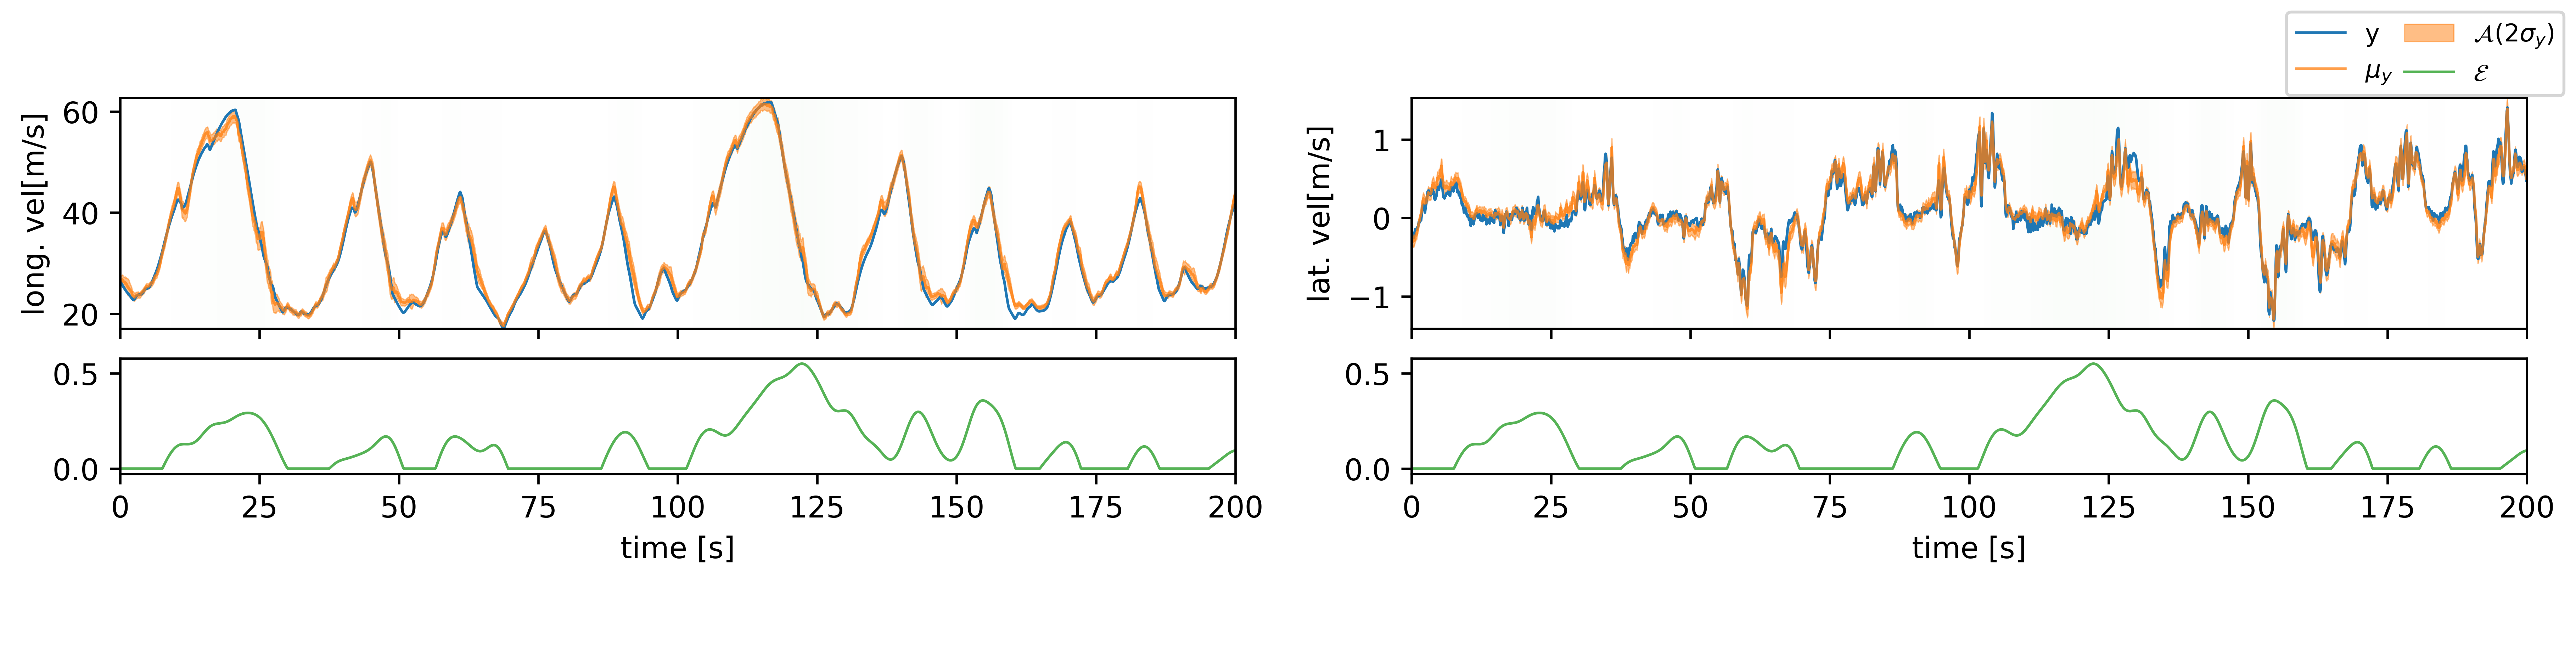
\includegraphics[width=\textwidth]{Experiments/figs/revs_test.png}
    \caption{Test}
  \end{subfigure}
  
  \begin{subfigure}[b]{\textwidth}
    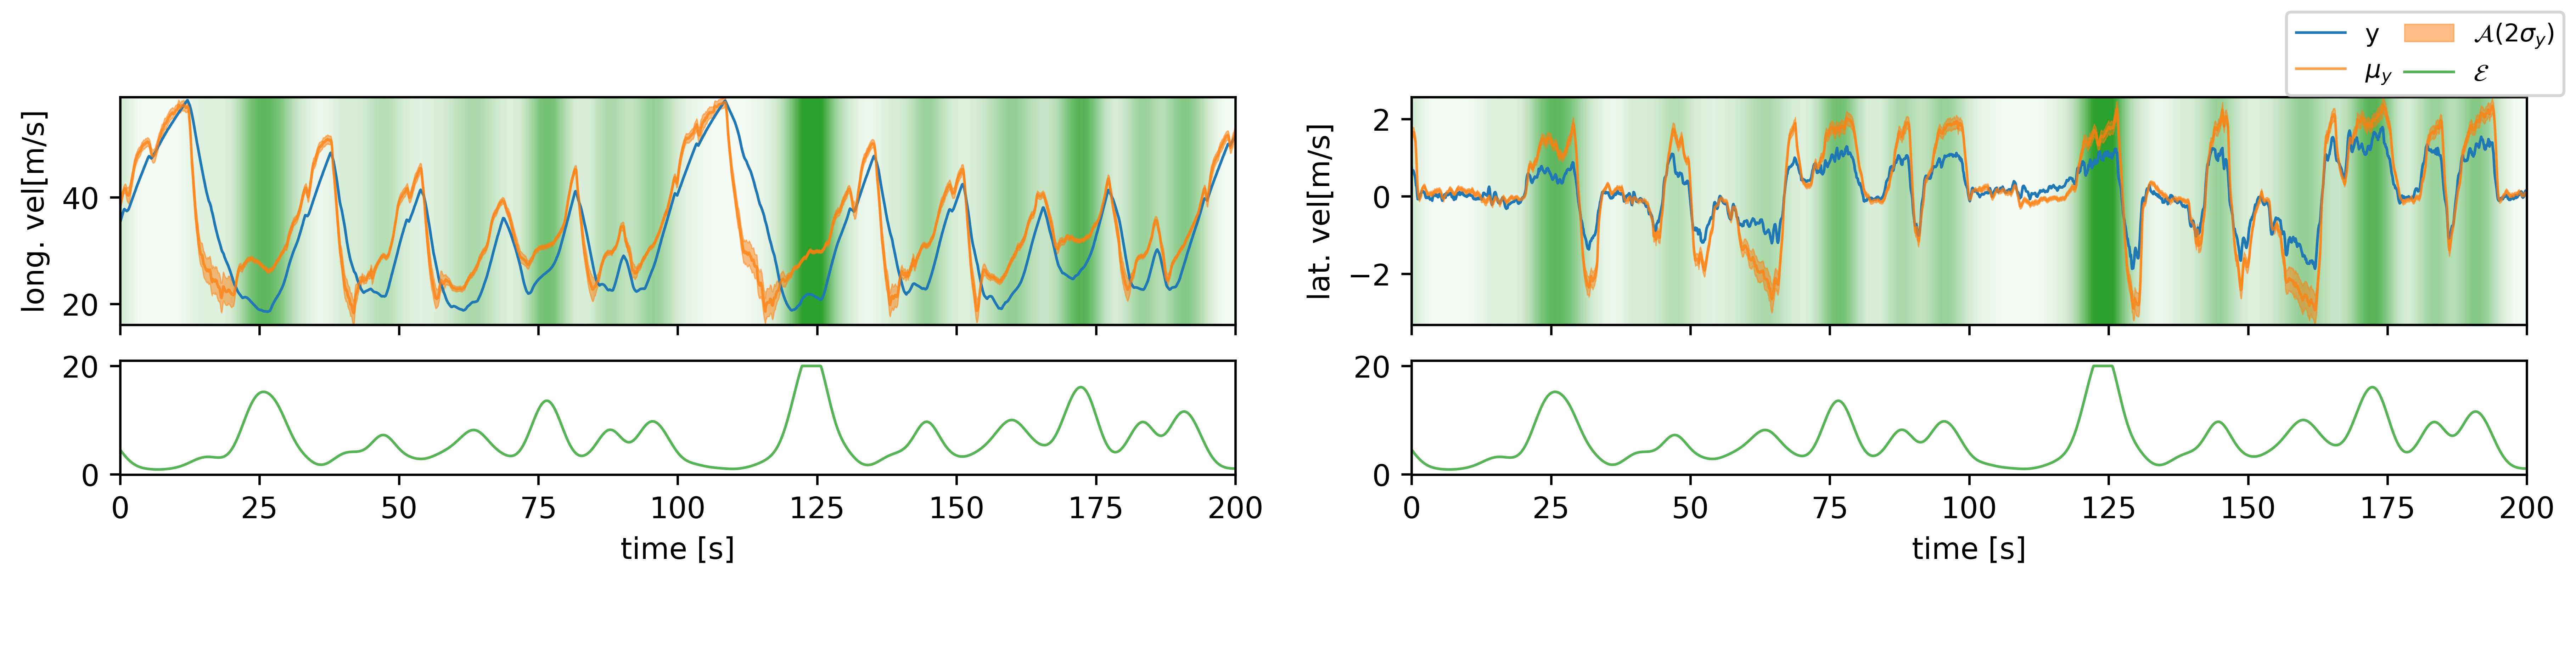
\includegraphics[width=\textwidth]{Experiments/figs/revs_ood.png}
    \caption{OOD}
  \end{subfigure}
  
  \caption{Revs test and ood plots for C-RNN. Aleatoric uncertainty represented as the shaded interval around the prediction(2 stds on each side). Epistemic Uncertainty plotted in the bottom row. The green shading also represents the epistemic uncertainty overlayed over the graph.}
  \label{fig:Revs_run}
\end{figure}


Those results are consistent with the expectation we set in \cref{ch:background}. First, it may seem surprising that the average aleatoric uncertainty does not go up at all over the OOD data, but as we said in \cref{subsec:aleatoric} model learns to estimate aleatoric uncertainty from the training data. In this light, it is not shocking that the average behavior does not change much across input regions. The model is simply matching the statistics it learned during training. The epistemic uncertainty, as we expected, does capture the errors coming from OOD inputs. 

\begin{table*}[htbp]
\centering
    \begin{tabular}{c  c  c}  
        \toprule
        Uncertainty score & AUROC$\uparrow$ & FPR@95\%$\downarrow$\\
        \midrule
        Aleatoric($\mathcal{A}$) & 0.47  & 0.90\\
        Epistemic($\mathcal{E}$) & 0.97 &  0.05 \\
        \midrule
    \end{tabular}
    \caption{OOD discrimination power of the aleatoric($\mathcal{A}$) and epistemic($\mathcal{E}$) uncertainties.}
    \label{tbl:revs_discrimination}
\end{table*}


\begin{table*}[htbp]
\centering
    \begin{tabular}{l l c c c c}  
        \toprule
        U. & Split & \multicolumn{2}{c}{MAE} & \multicolumn{2}{c}{$Zs$}\\
        \midrule
        & & $\rho \uparrow$ & $r \uparrow$ & $\rho \uparrow$ & $r \uparrow$ \\
        \multirow{3}{*}{$\mathcal{A}$} 
            & Test     & 0.57(0.51, 0.63) & 0.58(0.53, 0.62) & - & - \\  
            & OOD      & 0.49(0.36, 0.82) & 0.5(0.17, 0.83) & - & - \\  
            & Test+OOD & 0.39(0.16, 0.62) & 0.3(0.05, 0.54) & - & - \\ 

        \midrule
        \multirow{3}{*}{$\mathcal{E}$} 
            & Test     & 0.32  & 0.34 &  0.23  & 0.19 \\  
            & OOD      & 0.57 & 0.61 &  0.88 & 0.86 \\
            & Test+OOD & 0.85 & 0.80 &  0.93 & 0.91 \\ 

        \toprule
    \end{tabular}
    \caption{Pearson $\rho$ and Spearman $r$ correlations between the uncertainties and error scores. In the top half we check correlations with Aleatoric uncertainty, and in the bottom half with the epistemic uncertainty.}
    \label{tbl:revs_corr}
\end{table*}


To see how well our uncertainties can discriminate between the in/out-of-distribution data, we resort to the AUROC and FPR@95\% metrics. \cref{tbl:revs_discrimination} shows the results of those metrics when we use either the aleatoric or epistemic uncertainty to discriminate between test/OOD inputs. The results clearly show that the epistemic uncertainty does an excellent job at separating the two splits. Recall that the AUROC has a maximum of 1, and represents the probability that a random test input has lower uncertainty that a random OOD input. C-RNN's epistemic uncertainty puts that probability at 0.97. The aleatoric uncertainty is performing roughly on par with random behavior, which would have an expected 0.5 probability to give a test input lower score than an ood input.
To further understand the behavior and role of the uncertainties we need to look at correlations between errors and uncertainties. 


\Cref{tbl:revs_corr} shows the correlations between our error scores and uncertainties. The table is split such that the top half contains correlations between the errors and aleatoric uncertainty, and the bottom half between the errors and the epistemic uncertainty. For each uncertainty, we look at the correlations over the test and OOD splits separately, then combined.  

The aleatoric uncertainty shows the strongest correlations with the MAE over the test split alone, with an 0.57 Pearson coefficient. Within the OOD split alone the aleatoric uncertainty still shows good correlation with the MAE, with a Pearson correlation of 0.49. However, Over the combined splits, the correlation drops to 0.39. Given the fact that the average aleatoric uncertainty does not change between the test and OOD splits, while the MAE increases fivefold, it is not surprising that the correlation over the combined splits is low.

The epistemic uncertainty shows the reverse behavior for its correlation with the MAE, having the highest correlation over the combined splits with a Pearson coefficient of 0.85.  More notably, the epistemic uncertainty correlates strongly with the Z-score, as we would hope. We can see that it correlates weakly with he Z-score over the test split, correlates better over the OOD split, and best over the combined splits with a Pearson coefficient of 0.93 . 
Those results suggest that our model uncouples the uncertainties, to an extent, and each uncertainty is playing the role we expected. The aleatoric uncertainty focuses on errors within the test data, and the epistemic uncertainty focuses on errors coming from the OOD data. 

\Cref{fig:revs_uncertainty_corr} shows binned diagonal plots of the uncertainties versus our error scores over the combined splits. In those plots we perform quantile binning of the points according to the error score, then we plot the errors versus the uncertainty for the quantiles. The error bars in the plot represent the standard deviation of the uncertainty within each quantile. We use the MAE, Z-score, and the NLL as error scores. 

The plots show a separation of the points into a cluster of low error and a cluster of high error points. We can see from \cref{fig:revs_epistemic_corr} that the epistemic uncertainty clearly increases between the two groups. We can also see that over the high error points, it correlates well with the Z-score. 

The situation with the aleatoric uncertainty is complicated. We should again note that the aleatoric uncertainty is used in the calculation of both the NLL and the Z-score, as such we only include those plots for completeness, but we cannot offer a meaningful interpretation. Our focus for the aleatoric uncertainty is to observe its relationship with the MAE. We can see that for the low MAE points, the aleatoric uncertainty shows a correlation, but as we move farther into higher error regions, the correlation \emph{restarts}. Looking at the center plot of \cref{fig:revs_aleatoric_corr}, we can see that the aleatoric uncertainty correlates with the MAE separately within the a low and a high error interval. This is consistent with the numbers we see in \cref{tbl:revs_corr}, where we see that the correlation between aleatoric uncertainty and MAE is higher within the individual splits than when looking at the combined splits.

\begin{figure}[htbp]
  \centering
    \begin{subfigure}[b]{\textwidth}
        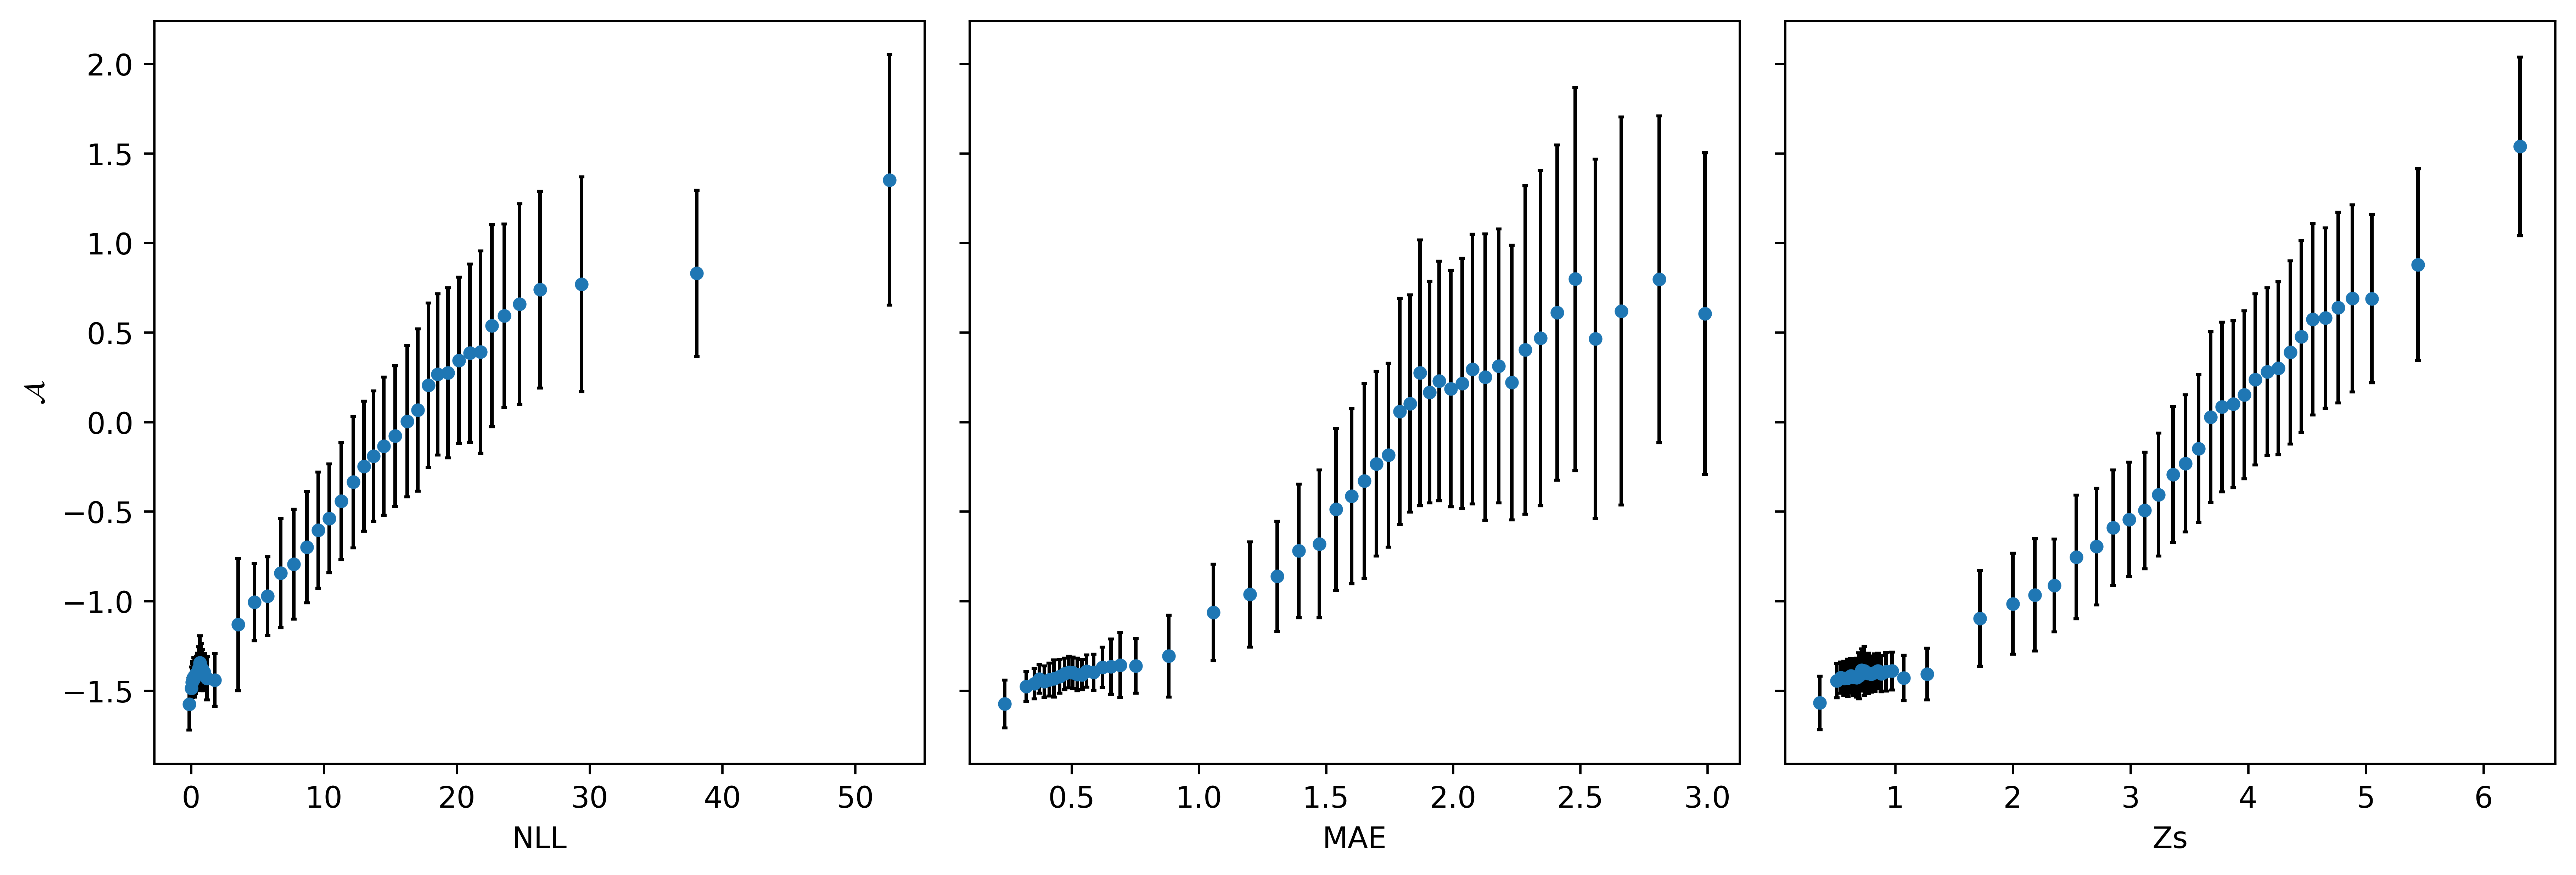
\includegraphics[width=\textwidth]{Experiments/figs/revs_epistemic_errors_corr.png}
        \caption{Binned diagonal plots for the epistemic uncertainty.}
        \label{fig:revs_epistemic_corr}
    \end{subfigure}
    
    \begin{subfigure}[b]{\textwidth}
        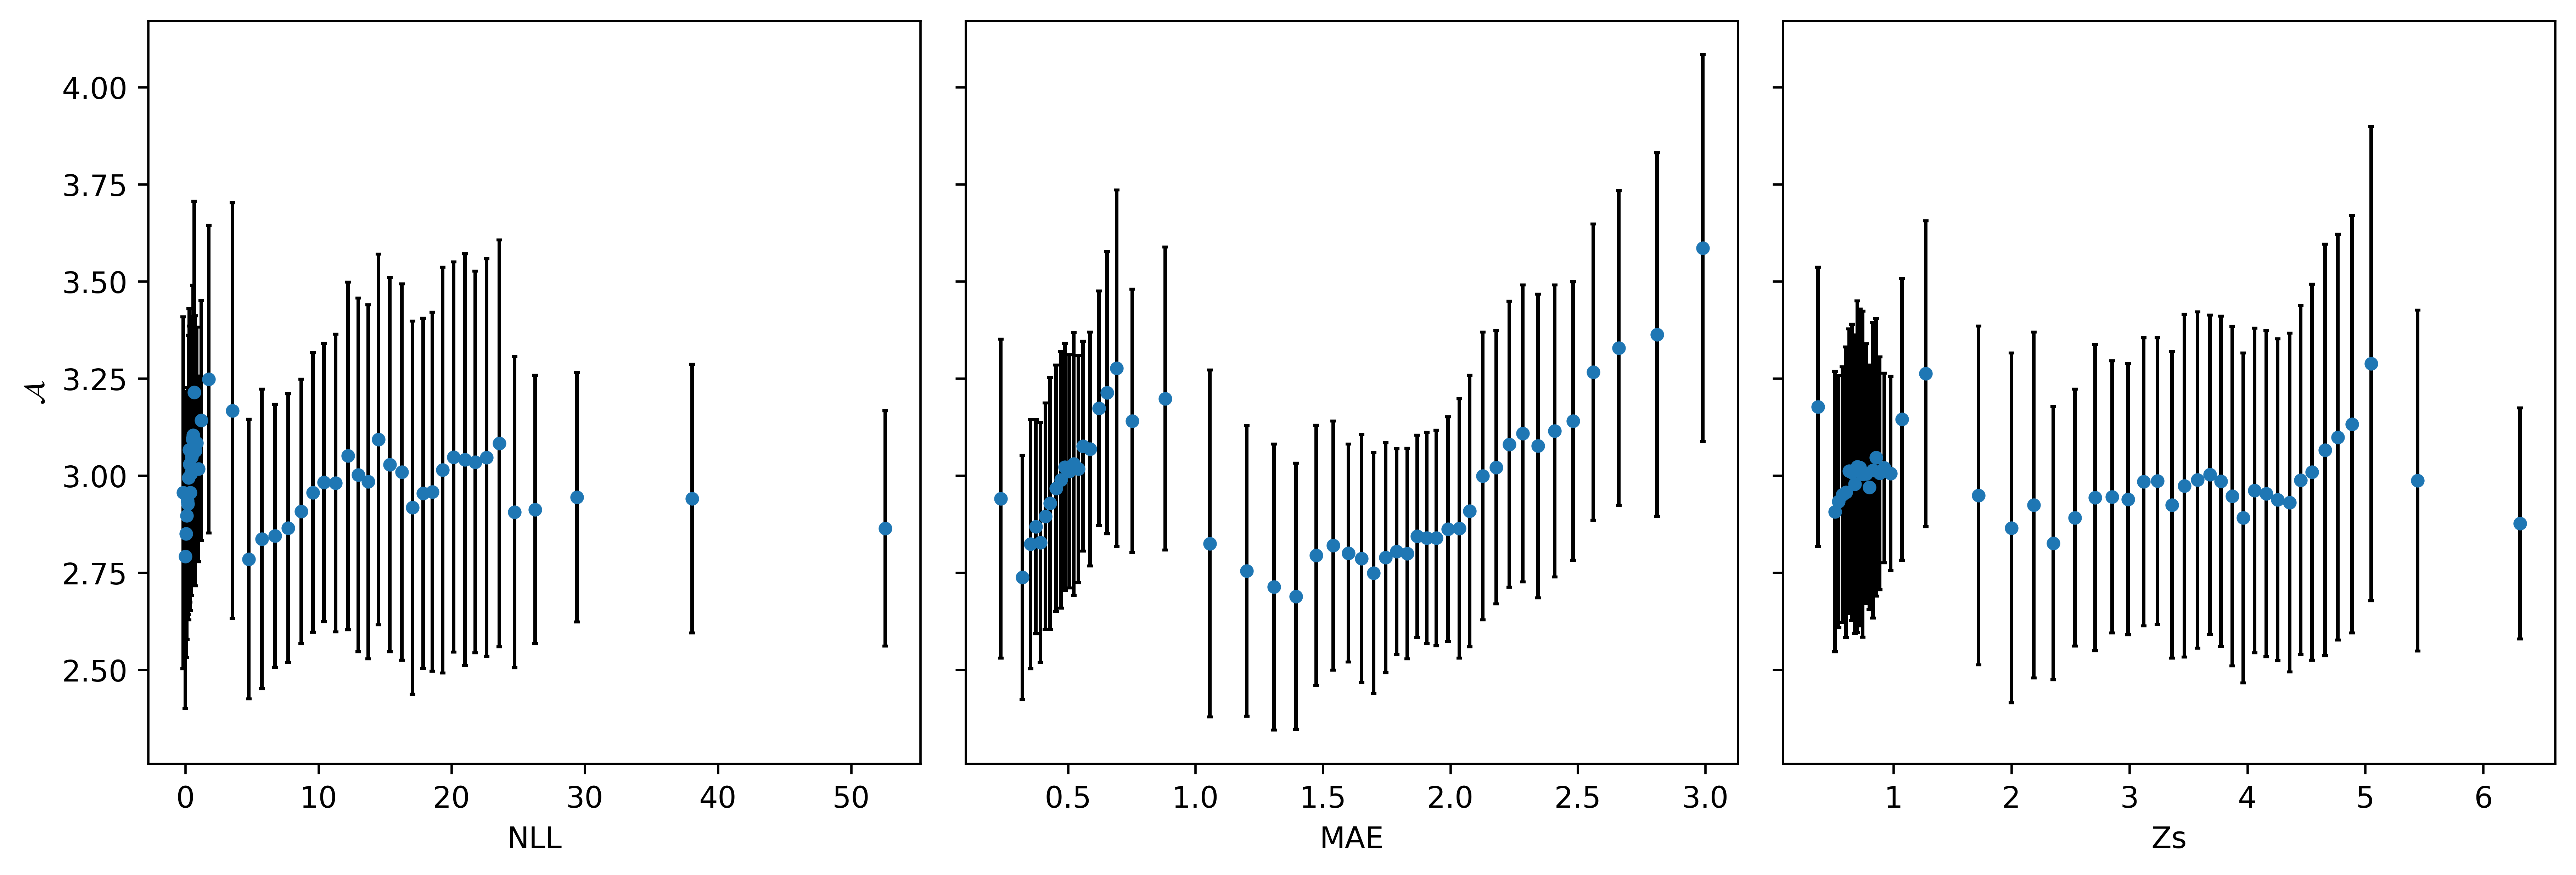
\includegraphics[width=\textwidth]{Experiments/figs/revs_aleatoric_errors_corr.png}
        \caption{Binned diagonal plots for the aleatoric uncertainty.}
    \label{fig:revs_aleatoric_corr}
  \end{subfigure}
    \caption{Revs binned diagonal plots of the  uncertainty vs our error scores over the combined splits(Test+OOD).}
    \label{fig:revs_uncertainty_corr}
\end{figure}


Lastly we wish to explore the relationship between our two uncertainties. We compute the correlations between the epistemic and aleatoric uncertainties. For the combined splits(Test+OOD), we get a Pearson correlation of 0.01 between the aleatoric and epistemic uncertainty. For the test split only, we get a Pearson of 0.014. For the OOD split only, we get Pearson 0.39. Again suggesting that for the C-RNN model the two uncertainties play different roles. 

\clearpage
\subsection{What about Dropout?}

MC dropout~\citep{gal2016dropout} is widely used as a tool to estimate epistemic uncertainty in deep learning. We have trained dropout models to see their behavior in our context. Recall that MC dropout is a variational approximation to the bayesian approach discussed in \cref{ch:background}~\citep{gal2016dropout}. 

The dropout models we train estimate the aleatoric uncertainty identically to our models, via outputting the mean and variance of a Gaussian. Thus the main difference is in the epistemic uncertainty estimation. Note that our approach and dropout are more orthogonal than competing. They focus on different source of uncertainty. Similar to the previous subsection, we will study the uncertainty dropout captures and how its two uncertainties interact with each other and the errors.

\begin{table*}[htbp]
\centering
    \begin{tabular}{c  c  c   c  c }  
        \toprule
        Split & MAE & NLL & $\mathcal{A}$ & $\mathcal{E}$\\
        \midrule
        Test &  1.26(2.4, 0.14) & 1.13(2.6, -0.37) & 2.38(4.5, 0.23) &  1.79(3.4, 0.14) \\
        OOD  &  2.55(4.9, 0.2)&  1.62(3.2, 0.02)& 2.42(4.6, 0.26)&  1.97(3.8, 0.16) \\
        \midrule
    \end{tabular}
    \caption{Revs MC dropout performance. The numbers are given with their std}
    \label{tbl:revs_dropout}
\end{table*}


\begin{figure}[htbp]
  \centering
  
  \begin{subfigure}[b]{\textwidth}
    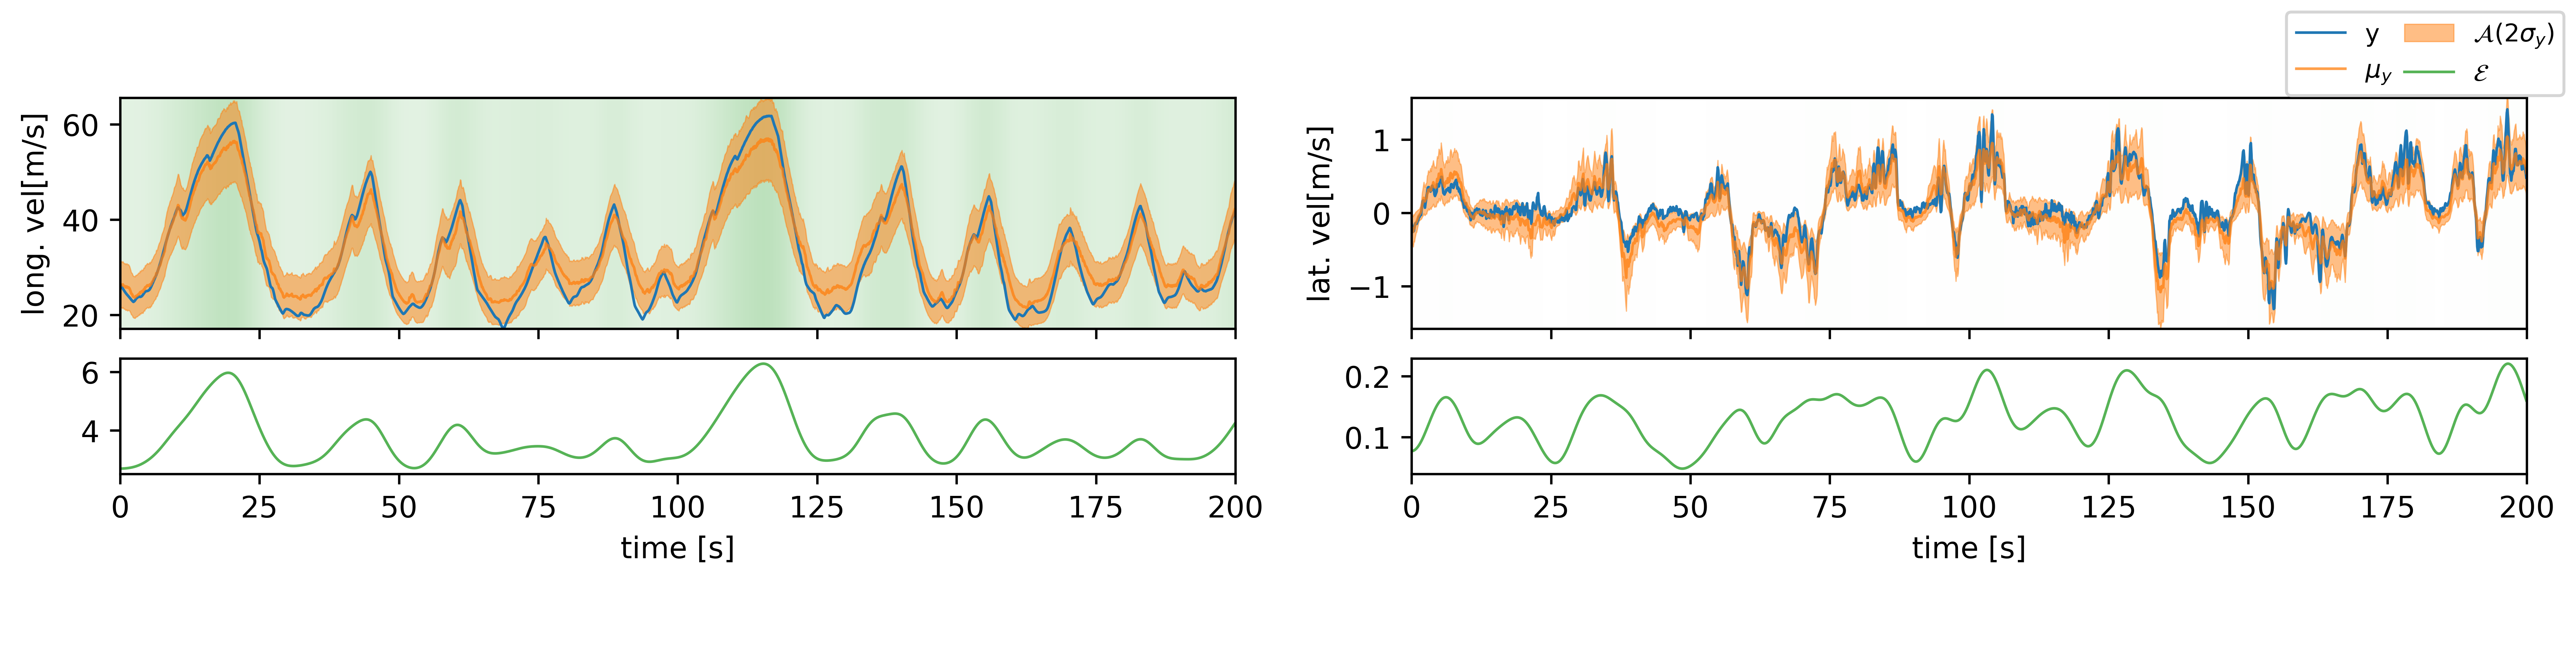
\includegraphics[width=\textwidth]{Experiments/figs/revs_dropout_test.png}
    \caption{Test}
  \end{subfigure}
  
  \begin{subfigure}[b]{\textwidth}
    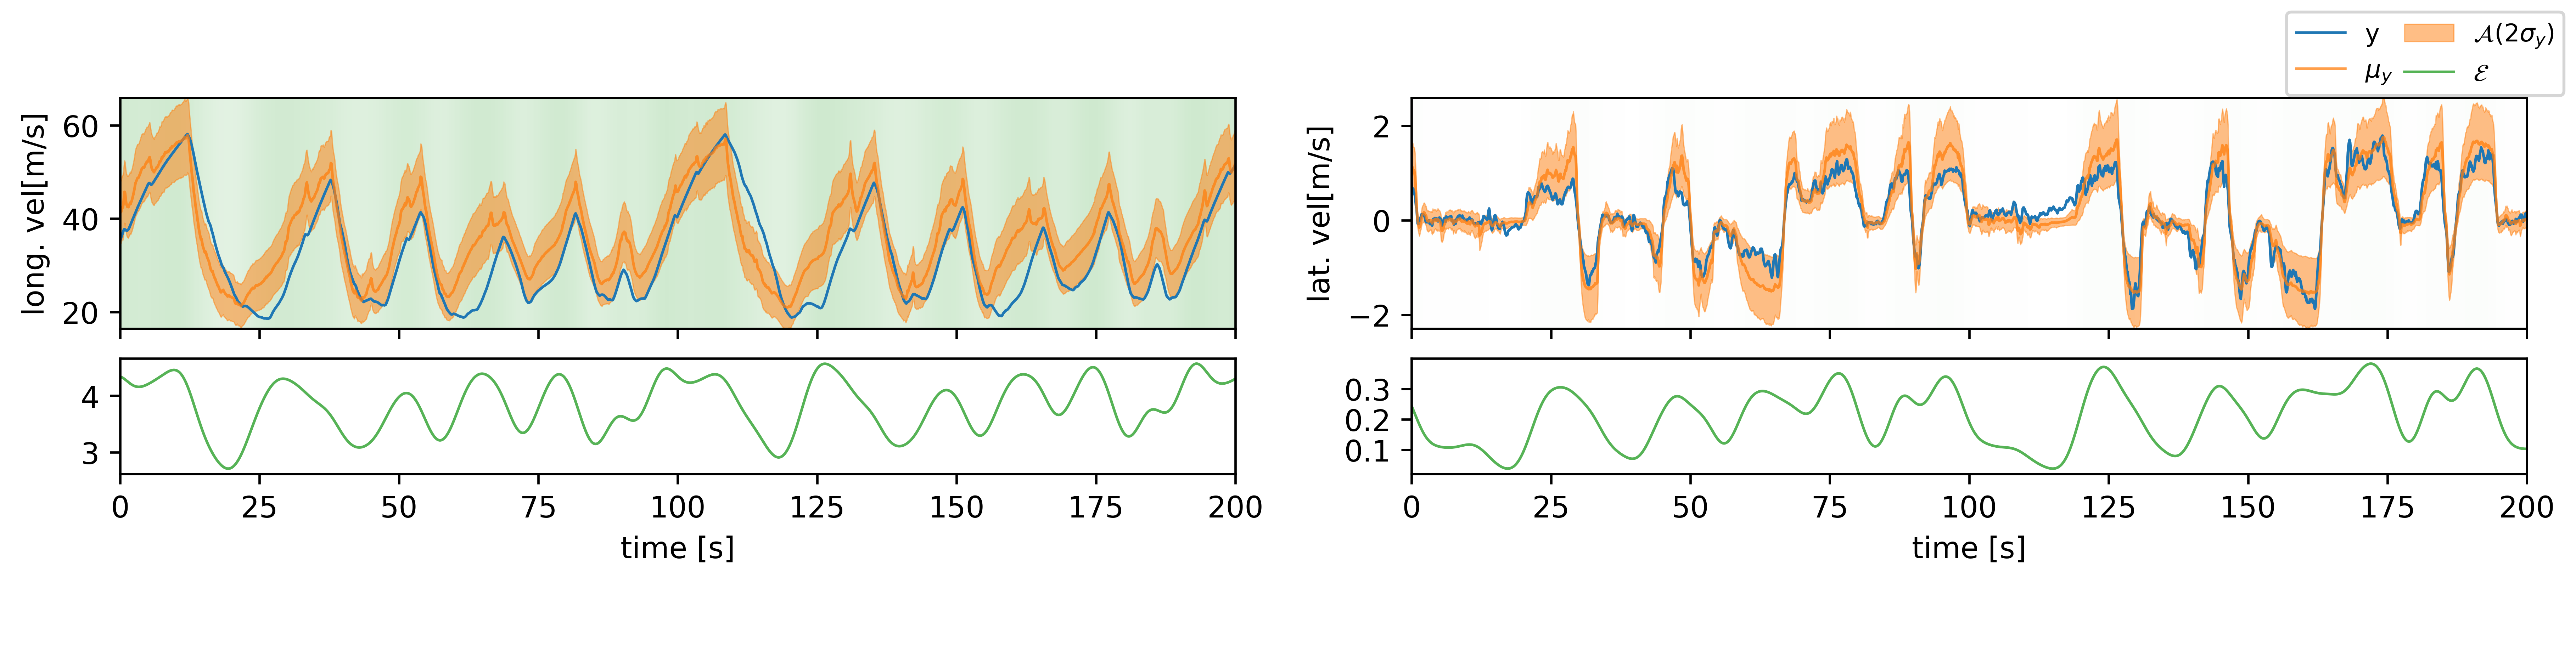
\includegraphics[width=\textwidth]{Experiments/figs/revs_dropout_ood.png}
    \caption{OOD}
  \end{subfigure}
  
  \caption{Revs test and ood prediction plots for MC dropout. Aleatoric uncertainty represented as the shaded interval around the prediction(2 stds on each side). Epistemic Uncertainty plotted in the bottom row. The green shading also represents the epistemic uncertainty overlayed over the graph.}
  \label{fig:revs_dropout_run}
\end{figure}

\Cref{fig:revs_dropout_run} shows prediction plots for the dropout model. Again we see that the model performance decreases over the OOD input. Another important thing to notice is that the epistemic uncertainty lies in the same range for both the test and OOD input. We will look at the numbers.

\Cref{tbl:revs_dropout} shows the basic results of MC dropout. Again we see that the MAE is higher on the OOD data, roughly a twofold increase from 1.26 to 2.55. However, this time we don't see as significant of an increase in the NLL between the test and OOD data. 
We still have that the aleatoric uncertainty does not change much between the splits. The epistemic uncertainty sees a slight increase on the OOD data, going from 1.79 over the test data to 1.97 for OOD. The numbers here suggest that the dropout model will not perform well in discriminating between the two splits.


\begin{table*}[htbp]
\centering
    \begin{tabular}{c  c  c}  
        \toprule
        Uncertainty score & AUROC$\uparrow$ & FPR@95\%$\downarrow$\\
        \midrule
        Aleatoric($\mathcal{A}$) & 0.57  & 0.93\\
        Epistemic($\mathcal{E}$) & 0.64 &  0.81 \\
        \midrule
    \end{tabular}
    \caption{Revs OOD discrimination power of the aleatoric($\mathcal{A}$) and epistemic($\mathcal{E}$) uncertainties for MC dropout.}
    \label{tbl:revs_dropout_discrimination}
\end{table*}


Again we evaluate how well the uncertainties from the dropout model can discriminate between the in/out-of-distribution points in \cref{tbl:revs_dropout_discrimination}. Again we see that the aleatoric uncertainty does no do well with an AUROC of 0.57, not far from 0.5, which is the expected AUROC for a random classifier. The epistemic uncertainty performs slightly better with an AUROC of 0.64. This is consistent with the numbers in \cref{tbl:revs_dropout}, where we saw that the uncertainties were on average the same for the test and OOD splits. This behavior is consistent with the argument we presented in \cref{ch:background}, that the Bayesian approach to learning, which MC dropout approximates, is not designed to deal with OOD data. 


\begin{table*}[htbp]
\centering
    \begin{tabular}{l l c c c c}  
        \toprule
        U. & Split & \multicolumn{2}{c}{MAE} & \multicolumn{2}{c}{$Zs$}\\
        \midrule
        & & $\rho \uparrow$ & $r \uparrow$ & $\rho \uparrow$ & $r \uparrow$ \\
        \multirow{3}{*}{$\mathcal{A}$} 
            & Test     & 0.46(0.17, 0.75) & 0.5(0.22, 0.77) & - & - \\  
            & OOD      & 0.25(-0.03, 0.54) & 0.31(-0.01, 0.63) & - & - \\  
            & Test+OOD & 0.32(0.03, 0.61) & 0.37(0.05, 0.69) & - & - \\ 

        \midrule
        \multirow{3}{*}{$\mathcal{E}$} 
            & Test     & 0.36(0.02, 0.71)  & 0.38(0.03, 0.74) &  -0.06(-0.14, 0.08)  & -0.02(-0.16, 0.11) \\ & OOD      & 0.32(0.11, 0.53) & 0.36(0.13, 0.6) &  0(0, 0) & 0.02(0.01, 0.03) \\
            & Test+OOD & 0.41(0.25, 0.58) & 0.42(0.27, 0.67) &  0.1(0.14, 0.05) & 0.14(0.17, 0.11) \\ 

        \toprule
    \end{tabular}
    \caption{Revs Pearson $\rho$ and Spearman $r$ correlations between the uncertainties and error scores for MC dropout. In the top half we check correlations with Aleatoric uncertainty, and in the bottom half with the epistemic uncertainty.}
    \label{tbl:revs_dropout_corr}
\end{table*}

In \cref{tbl:revs_dropout_corr} we show the correlations between MC dropout uncertainties and errors in order to better understand what uncertainties the dropout model captures. 
Starting with the aleatoric uncertainty, we can see that it correlates best with the MAE over the test split, as is to be expected, with an average Pearson coefficient of 0.46, over the combined splits we get a weaker Pearson coefficient of 0.32. 

For the epistemic uncertainty, we see a correlation between the uncertainty and the MAE, which is highest over the combined splits with an 0.41 average Pearson coefficient. One noteworthy pattern for MC dropout is the lack of correlation between the epistemic uncertainty and the Z-score. Recall that the Z-score is the ratio of the absolute error to the aleatoric uncertainty. We introduce the Z-score to measure how well epistemic uncertainties capture errors which are not captured by the aleatoric uncertainty. Here we see that the epistemic uncertainty correlates with the MAE, but not with the Z-score. This suggests that the epistemic uncertainty captures the same errors as the aleatoric uncertainty. 

In fact, when we compute the correlation between the epistemic and aleatoric uncertainty for MC dropout we find a Pearson coefficient of 0.79 for the combined splits, 0.77 for the test split, and 0.8 for the OOD split. Note that this correlation between epistemic and aleatoric uncertainties for MC dropout has also been observed by \cite{kendall2017uncertainties}.


\subsection{Key points}

In this section, we will start by summarizing the key points from the in-depth results we just saw from our C-RNN model and MC dropout. Then we will show direct comparison of the key performance measures for the two models.

Our key findings 

\begin{itemize}
    \item The epistemic uncertainty estimated by the C-RNN model is effective in discriminating between in and out-of-distribution samples.
    
    \item The epistemic uncertainty estimated by MC dropout is not effective in discriminating between in and out-of-distribution samples.
    
    \item The aleatoric uncertainty behaves similarly in both models and is not effective in discriminating between the in and out-of-distribution samples.
    
    \item For the C-RNN model the epistemic and aleatoric uncertainties are not correlated and provide different types of information.
    
    \item For the MC dropout model the epistemic and aleatoric uncertainties are highly correlated and provide the same information. 
\end{itemize}{}


\begin{table*}[htbp]
\centering
    \begin{tabular}{l l c c c c c}  
        \toprule
        Model & split & MAE & NLL & $\rho$(MAE vs $\mathcal{E}$) &
        $\rho$(Z-score vs $\mathcal{E}$) & AUROC($\mathcal{E}$)\\
        \midrule
        \multirow{3}{*}{C-RNN} 
            & Test     & 0.55& 0.44 & 0.32  & 0.23 & - \\  
            & OOD      & 2.6 & 17.8 & 0.57  & 0.88 & -\\  
            & Test+OOD & 1.6 & 9.2  & 0.85  & 0.93 & 0.97\\ 

        \midrule
        \multirow{3}{*}{MC dropout} 
            & Test     & 1.26 & 1.14  & 0.36  & -0.06 & - \\  
            & OOD      & 2.55 & 1.62  & 0.32  & 0 & -\\  
            & Test+OOD & 1.8  & 1.38  & 0.42  & 0.1 & 0.64\\ 

        \toprule
    \end{tabular}
    \caption{Revs key results for comparison of C-RNN and MC dropout. $\rho$ is the Pearson correlation.}
    \label{tbl:revs_comparison}
\end{table*}


\Cref{tbl:revs_comparison} contains a summary of the key results for comparison between C-RNN and MC dropout. The main difference between the two models is the approach to estimating the epistemic uncertainty. We can see that C-RNN's epistemic uncertainty performs significantly better in discriminating between the in and out-of-distribution points with an AUROC of 0.97 compared to MC dropout's 0.64.

Looking at how the uncertainty correlates with the errors, we can see that over the combined splits C-RNN performs better for both the MAE and the Z-score. C-RNN's epistemic uncertainty has an 0.93 correlation with the Z-score while MC dropout has a correlation of 0.1.Over the test split alone MC dropout shows a correlation of 0.32 between the epistemic uncertainty and the MAE, and -0.06 between the epistemic uncertianty and the Z-score. On the other hand, C-RNN shows a correlation of 0.32 between the epistemic uncertainty and the MAE, and 0.23 between the epistemic uncertainty and the Z-score. Thus even in the setting where OOD data is excluded C-RNN's epistemic uncertainty correlates better with the Z-score.    
 



\subsubsection{Ablations}

\begin{table*}[htbp]
\centering
    \begin{tabular}{l l c c c c }  
        \toprule
        Model & split & MAE & NLL & $\rho$(MAE vs $\mathcal{E}$) &
        $\rho$(Z-score vs $\mathcal{E}$)\\
        \midrule
        \multirow{3}{*}{C-RNN(no annealing)} 
            & Test     & 0.69 & 0.63 & 0.48  & 0.15\\  
            & OOD      & 3.07 & 9.91 & 0.58  & 0.44\\  
            & Test+OOD & 1.9  & 5.2  & 0.66  & 0.59\\ 

        \midrule
        \multirow{3}{*}{C-RNN(no weighting)} 
            & Test     & 0.55 & 0.42  & 0.48  & 0.2\\  
            & OOD      & 2.51 & 7.66  & 0.42  & 0.4 \\  
            & Test+OOD & 1.6  & 4.04  & 0.77  & 0.77\\ 
            
        \midrule
        \multirow{3}{*}{C-RNN} 
            & Test     & 0.55& 0.44 & 0.32  & 0.23\\  
            & OOD      & 2.6 & 17.8 & 0.57  & 0.88\\  
            & Test+OOD & 1.6 & 9.2  & 0.85  & 0.93\\ 

        \toprule
    \end{tabular}
    \caption{Revs ablation study}
    \label{tbl:revs_ablation}
\end{table*}


Our last set of results with the Revs dataset is going to be an ablation study, showing the effect of the additional components we use to train C-RNN, namely the KL annealing and the compression loss weighting. 

In \cref{tbl:revs_ablation} we show the key results for our full C-RNN model versus ablated versions. We show two ablated versions of the model one trained without the KL annealing and one trained without the compression loss weighting, along with the our full model.

Recall our motivation for adding the KL annealing to our model is to prevent a form of under-fitting caused by the model trying to minimize the penalty of encoding information in the latent state. In the top part of \cref{tbl:revs_ablation} we show the performance of C-RNN trained without KL annealing. We can see that the test MAE is higher with 0.69 versus 0.55 for the standard full C-RNN. The correlation of the epistemic uncertainty with the errors is also lower. For instance the correlation with the Z-score is 0.59 for the combined split, whereas the full model has a correlation of 0.93 in that setting. 

In the middle part of the model we have the results for a C-RNN trained without our compression loss weighting scheme. Recall that we introduced this scheme to increase the correlation between the epistemic uncertainty and the Z-score. We can see from the table that this is exactly what happens with the standard model having a correlation of 0.93 between the epistemic uncertainty and the Z-score, the model trained without the weighting scheme has a correlation of 0.77. 




With this ablation study we conclude our in-depth analysis and work on the revs dataset. In the next section we will present result using a different dataset in order to further validate the findings and insights we presented in this section. 

\clearpage
\section{Blackbird(1) results}
In the following set of experiments with the Blackbird dataset, we split the data into in/out-of-distribution by trajectory. Recall that the datasets consists of 163 unique flight sequences, and each sequence follows one of seventeen trajectories. We select four challenging trajectories as OOD and exclude all their sequences from the training data, details of the split available in \cref{app:blkbrd_split}. 

As we will see in the results, with this split the models can generalize well to the OOD inputs, despite the fact that the probability of those inputs is zero under the training distribution. This provides a different setting from the one we saw in the last section, where model errors increased for the OOD data.

This section will follow the same structure as the previous one, but will proceed faster and focus on validating the key findings. 

\subsection{C-RNN analysis}

\begin{table*}[h]
\centering
    \begin{tabular}{c  c  c   c  c }  
        \toprule
        Split & MAE & NLL & $\mathcal{A}$ & $\mathcal{E}$\\
        \midrule
        Test & 0.3(0.29, 0.31) & 0.3(0.27, 0.33) & 0.31(0.3, 0.32) &  -6.1\\
        OOD  &  0.27(0.25, 0.29) &  0.13(0.03, 0.22) & 0.28(0.27, 0.29)&  -6.2\\
        \midrule
    \end{tabular}
    \caption{Blackbird(1) C-RNN performance.}
    \label{tbl:bb1_CRNN}
\end{table*}

% \begin{figure}[h]
%   \centering
  
%   \begin{subfigure}[b]{\textwidth}
%     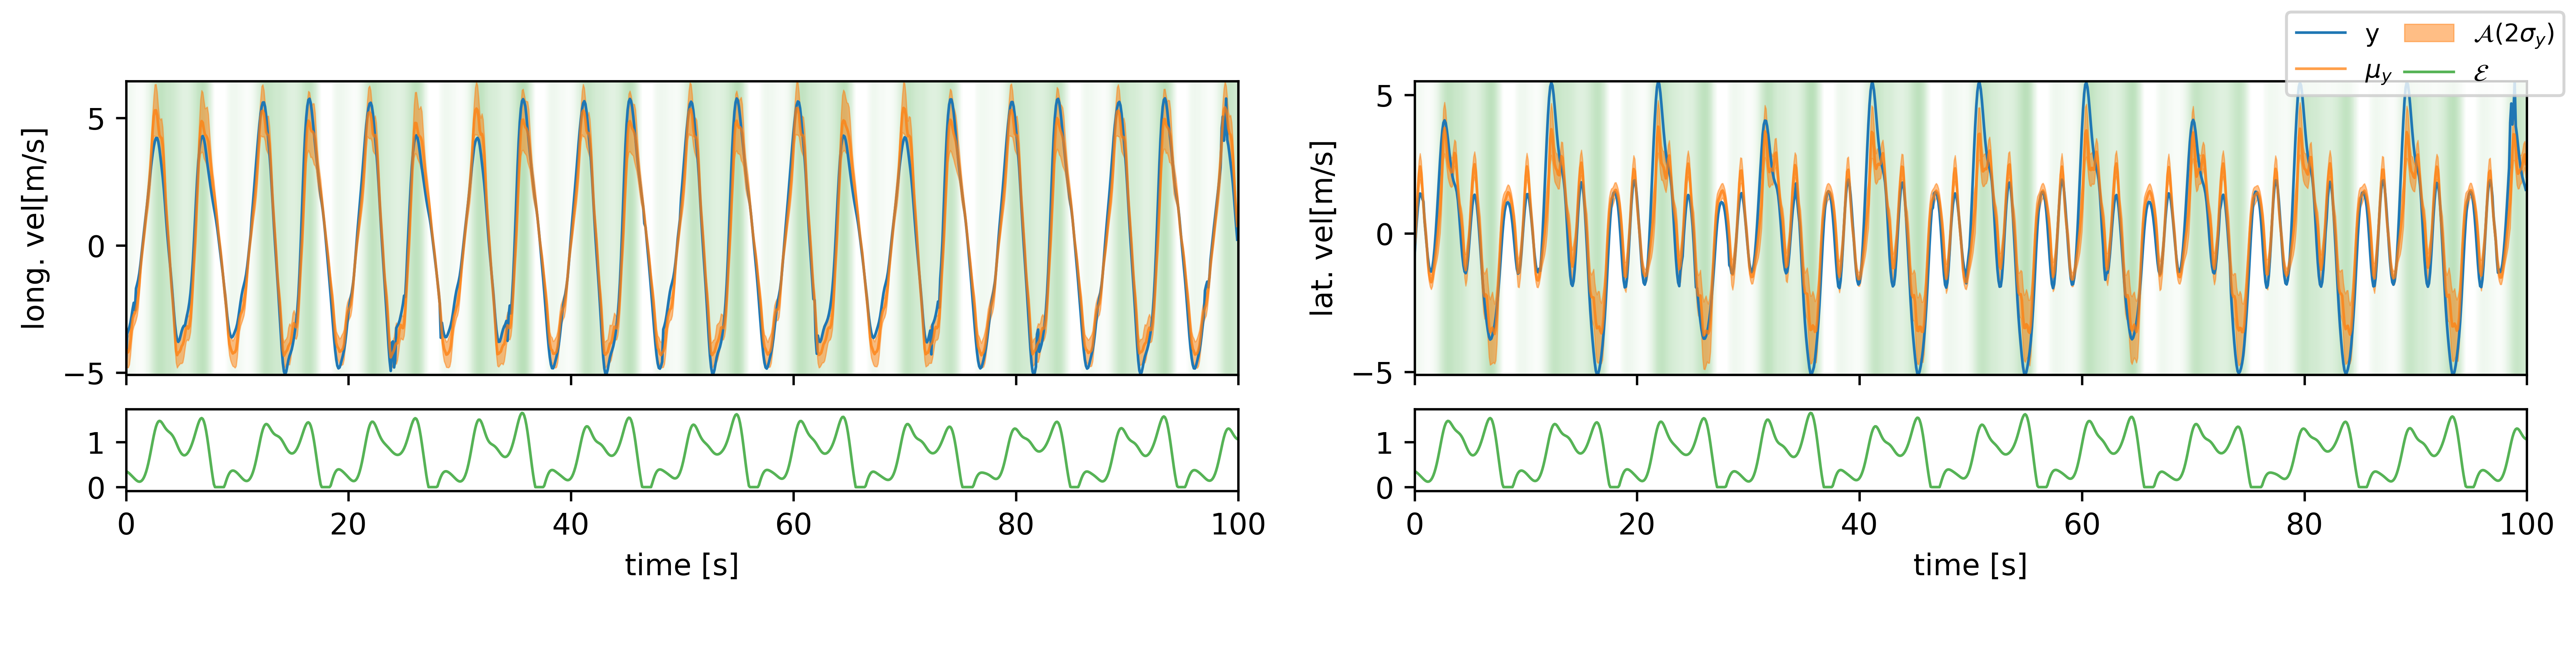
\includegraphics[width=\textwidth]{Experiments/figs/bb1_test.png}
%     \caption{Test}
%   \end{subfigure}
  
%   \begin{subfigure}[b]{\textwidth}
%     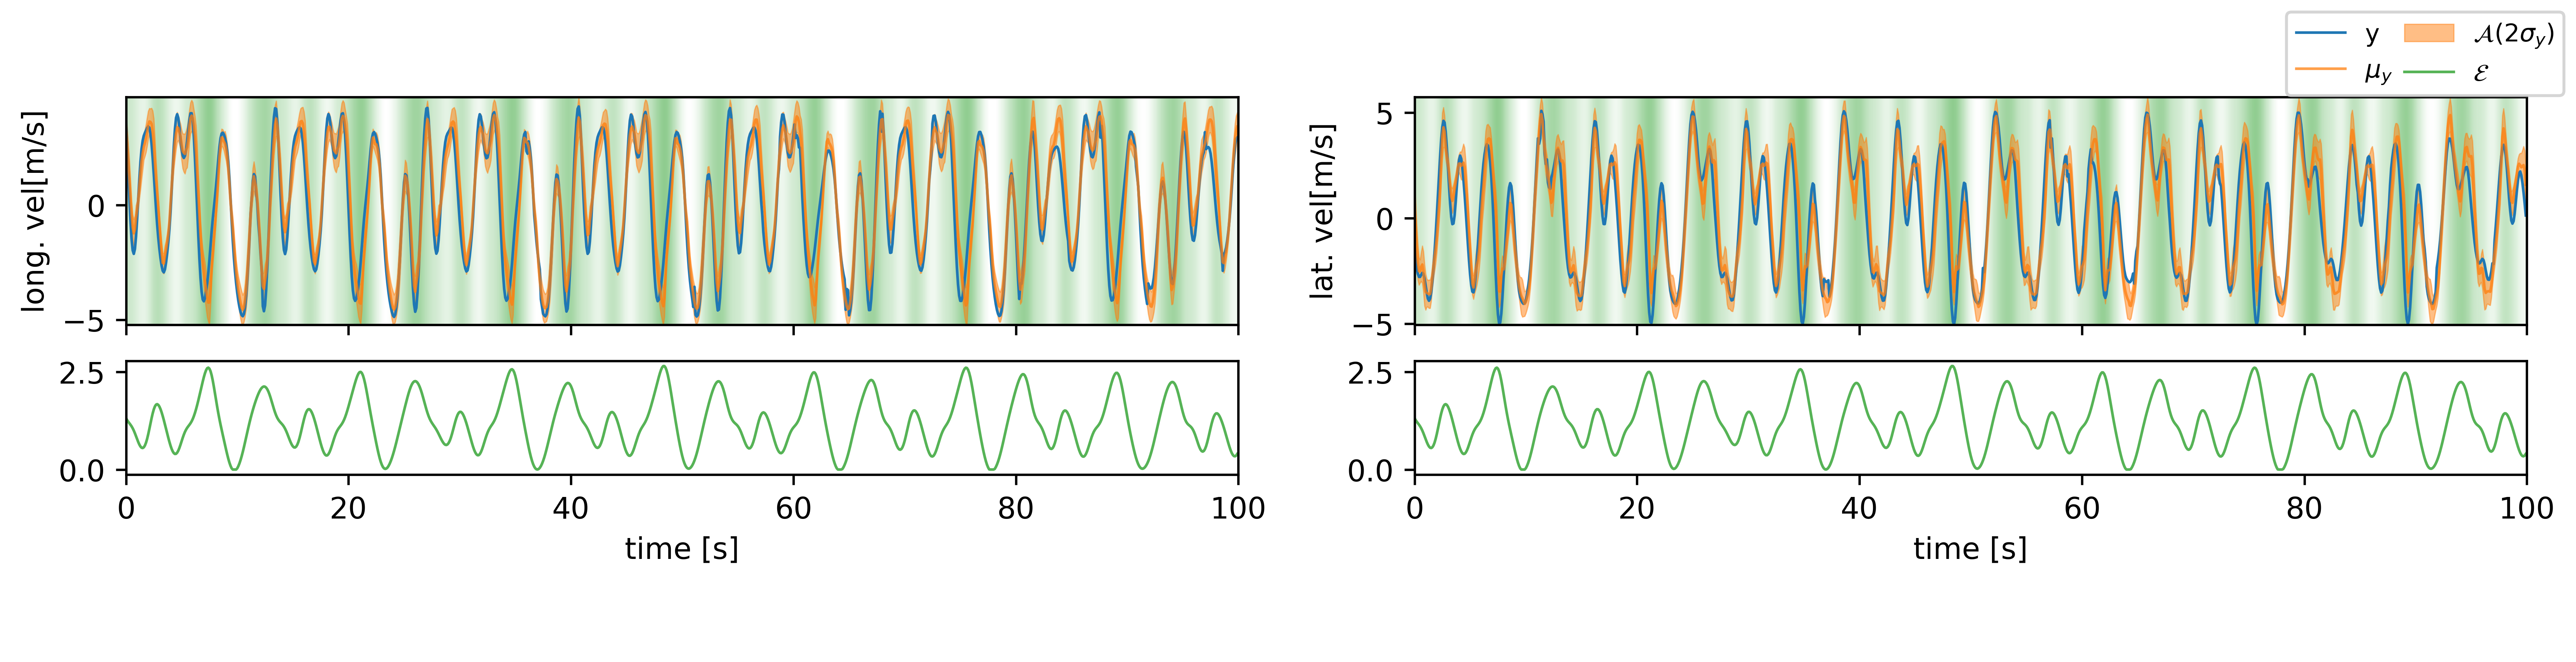
\includegraphics[width=\textwidth]{Experiments/figs/bb1_ood.png}
%     \caption{OOD}
%   \end{subfigure}
  
%   \caption{Blackbird(1) prediction plots for C-RNN.}
%   \label{fig:bb1_run}
% \end{figure}

\Cref{fig:bb1_run} shows a flight sequence with the model predictions for a test and an OOD input. We can see from the plots that the model behavior and quality of predictions is quite similar for the two sequences. In \cref{tbl:bb1_CRNN} we can see that the performance of C-RNN is similar for the two splits.

This is a tricky setting, since the model's errors are not correlated with the input being in or out-distribution. Recall that being out-of-distribution simply means the probability of the input is zero under the training distribution, this does not automatically imply that the model won't be able to generalize to some of those inputs. In fact we can see here that the model generalizes quite well, even giving a lower NLL of 0.13 for the OOD split, compared to 0.3 over the test split. In this case, we would not want our epistemic uncertainty to be high for OOD inputs in general, but rather to correlate with the errors. 
Fortunately, we can already see in \cref{tbl:bb1_CRNN} that the epistemic uncertainty on average is roughly the same for both splits. 

This setting shows how metrics such as AUROC which are widely used in works for OOD detection~\citep{liang2017enhancing, hein2019relu, lee2017training} are only meaningful if we assume that the model performs poorly on the OOD data we have. We have shown in the previous section that C-RNN's epistemic uncertainty estimates did an excellent job separating the in/out-of-distribution points with an AUROC of 0.97. In this setting, our C-RNN has an AUROC of 0.46, which is close to random behavior. This is a desirable result in this case, since there is no reason for the uncertainty to be higher in general on the OOD inputs if the errors are not.


\begin{table*}[h]
\centering
    \begin{tabular}{l l c c c c}  
        \toprule
        U. & Split & \multicolumn{2}{c}{MAE} & \multicolumn{2}{c}{$Zs$}\\
        \midrule
        & & $\rho \uparrow$ & $r \uparrow$ & $\rho \uparrow$ & $r \uparrow$ \\
        \multirow{3}{*}{$\mathcal{A}$} 
            & Test     & 0.81(0.81, 0.81) & 0.81(0.78, 0.84) & - & - \\  
            & OOD      & 0.86(0.9, 0.81) & 0.88(0.89, 0.87) & - & - \\  
            & Test+OOD & 0.84(0.87, 0.80) & 0.86(0.86, 0.86) & - & - \\ 

        \midrule
        \multirow{3}{*}{$\mathcal{E}$} 
            & Test     & 0.88  & 0.86 &  0.31  & 0.41 \\  
            & OOD      & 0.90 & 0.89 &  0.51 & 0.64 \\
            & Test+OOD & 0.88 & 0.86 &  0.44 & 0.57 \\ 

        \toprule
    \end{tabular}
    \caption[Blackbird(1) error-uncertainty correlation for C-RNN]{Blackbird(1) Pearson $\rho$ and Spearman $r$ correlations between the uncertainties and error scores for C-RNN.}
    \label{tbl:bb1_corr}
\end{table*}

Our best test for quality of the uncertainty estimates in this case is their correlation with the errors. \Cref{tbl:bb1_corr} shows the correlations between our error scores and uncertainties.  Here we note that both the aleatoric and epistemic uncertainty correlate highly with the MAE. The aleatoric uncertainty has a Pearson correlation of 0.84 with the MAE, and the epistemic uncertainty has a correlation of 0.88 with the MAE. 

The high correlation of the epistemic uncertainty with the errors is good news, given that we are in the context where OOD data have the same MAE as the in-distribution data. However, the strong correlation of the aleatoric and epistemic uncertainty with the MAE suggests that they may be giving the same information. Indeed we find that the Pearson correlation between the epistemic and aleatoric uncertainty to be 0.95. Thus in the particular setting here we see redundancy between our two uncertainty estimates, but on a positive note they both correlate with the errors well, and we at least don't see our model assign overly high uncertainties to the OOD inputs. Recall that in the Revs dataset, C-RNN assigned much larger uncertainties to the OOD data with an average -0.25 epistemic uncertainty for the OOD data and an average -4.6 epistemic uncertainty to the test data. Thus on a positive note, the model is flexible enough to cope with both situations. 

\begin{figure}[htbp]
  \centering
    \begin{subfigure}[b]{\textwidth}
        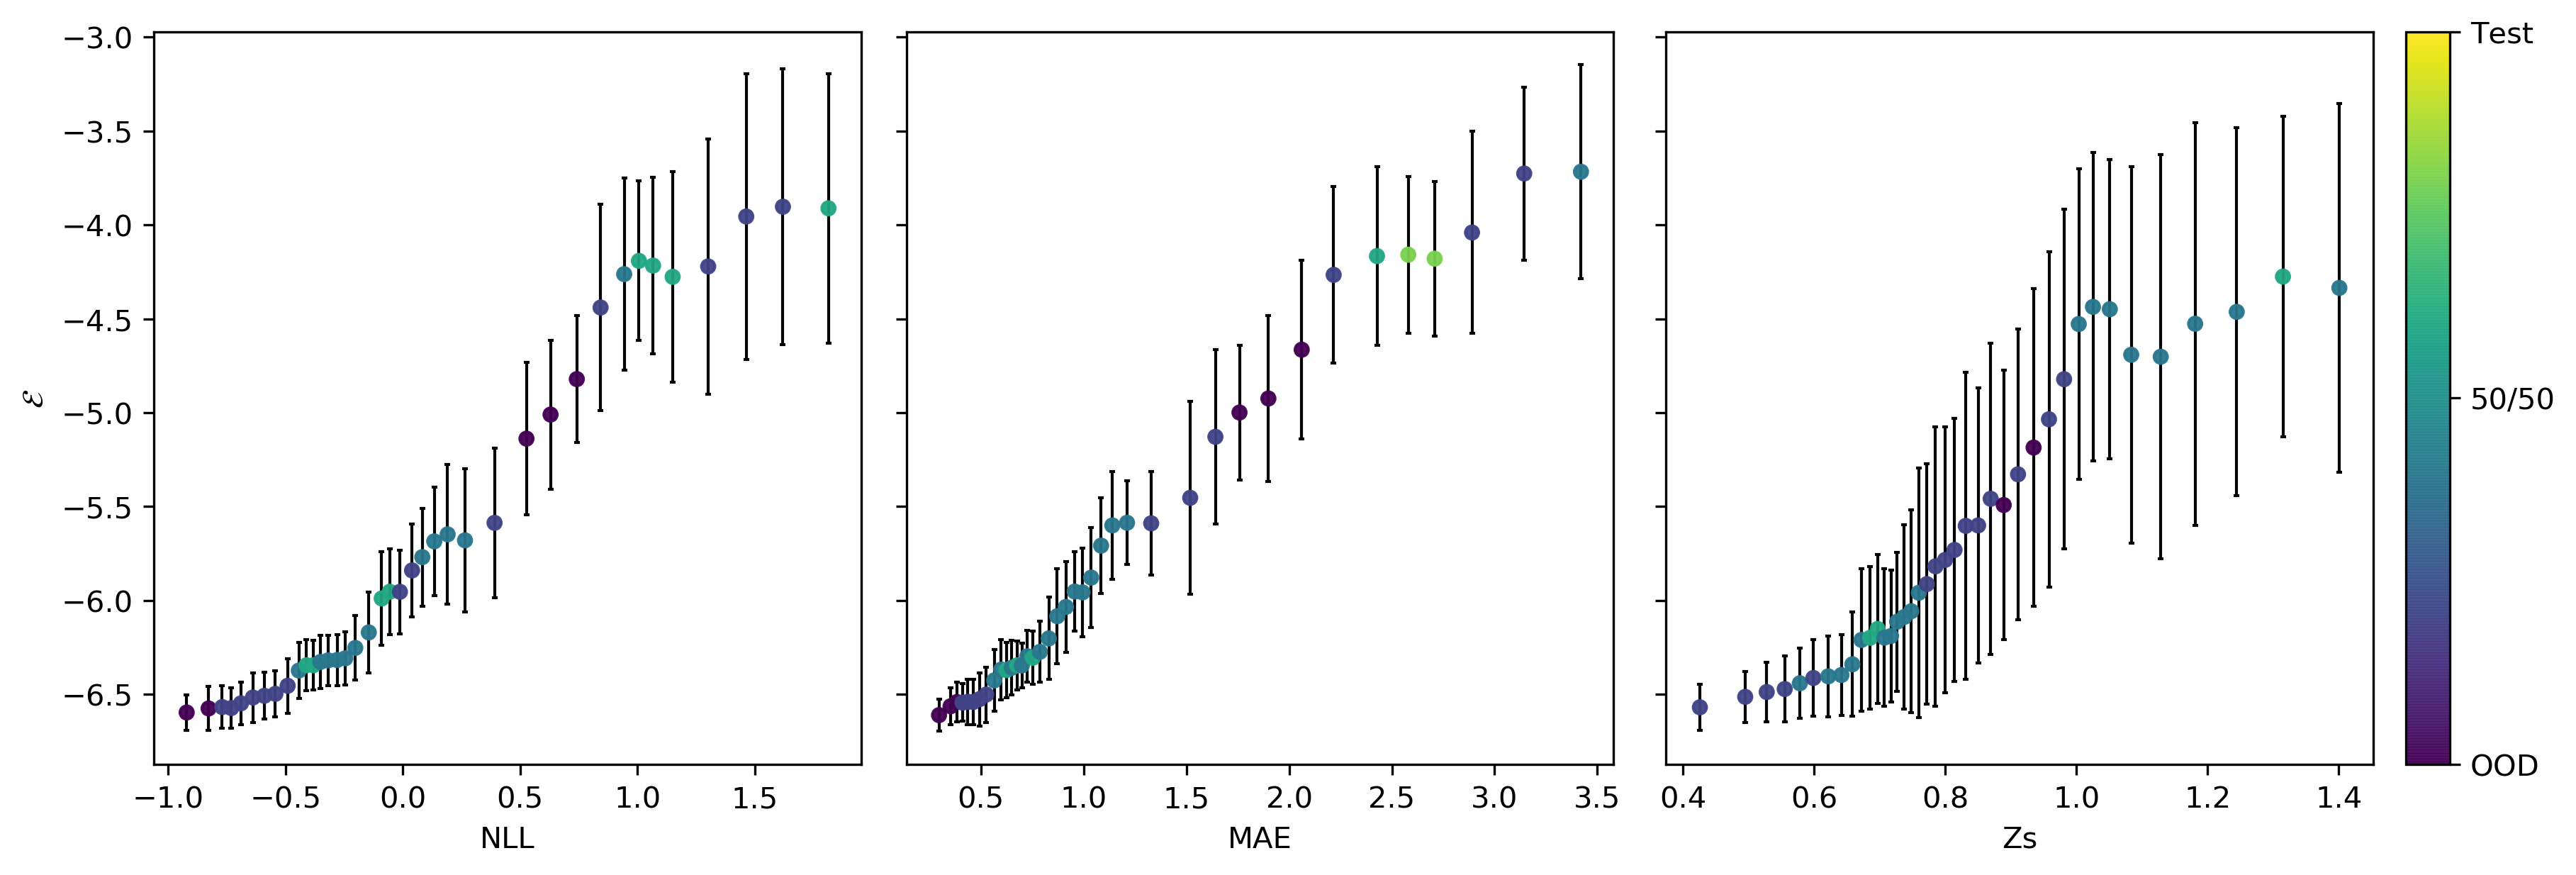
\includegraphics[width=\textwidth]{Experiments/figs/binned/bb1_crnn_epistemic.png}
        \caption{Binned diagonal plots for the epistemic uncertainty.}
    \end{subfigure}
    
    \begin{subfigure}[b]{\textwidth}
        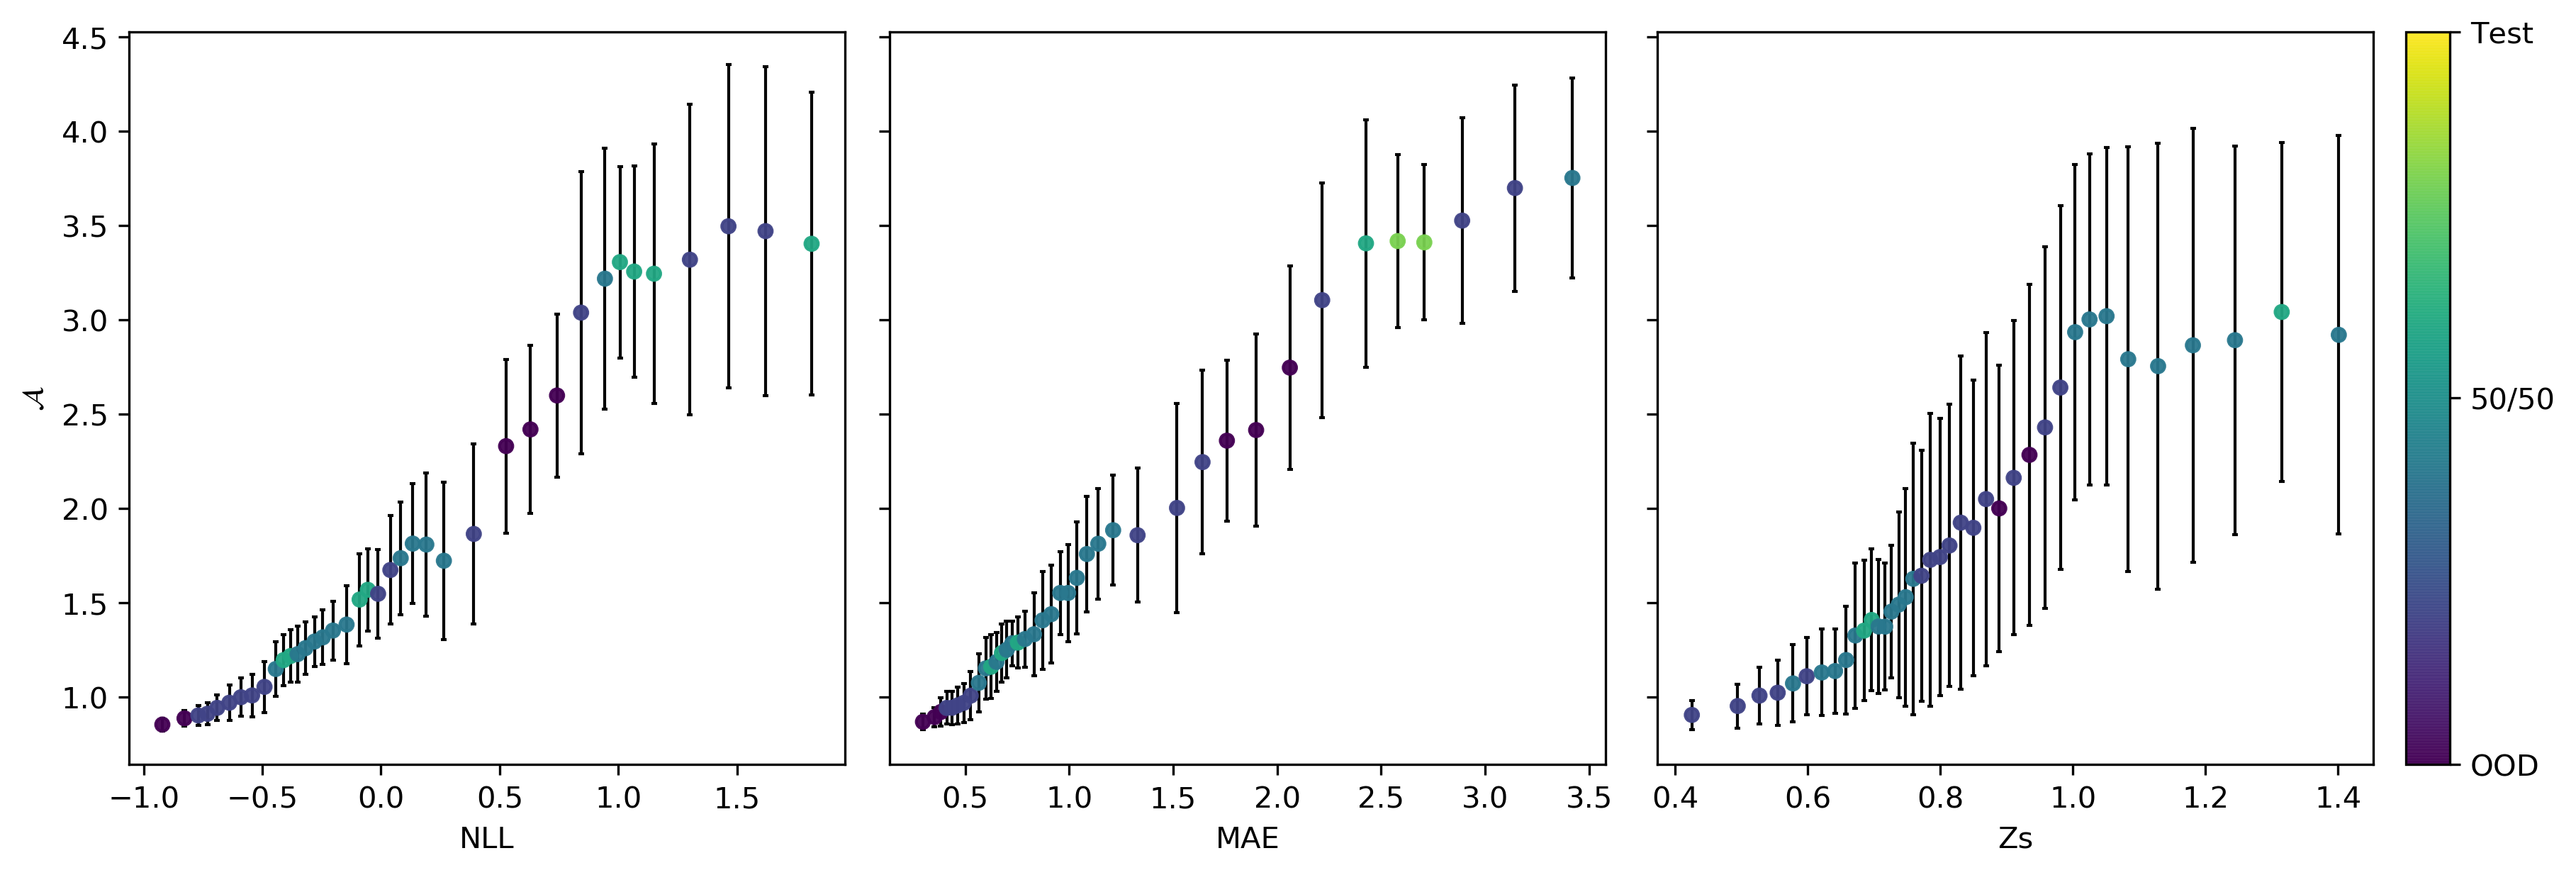
\includegraphics[width=\textwidth]{Experiments/figs/binned/bb1_crnn_aleatoric.png}
        \caption{Binned diagonal plots for the aleatoric uncertainty.}
  \end{subfigure}
    \caption[Blackbird(1) error-uncertainty diagonal plots for C-RNN]{Blackbird(1) binned diagonal plots of the  uncertainty vs error scores(NLL, MAE, Z-score) over the combined splits(Test+OOD). The marker color denotes the ratio of test to OOD points in the bin. }
    \label{fig:bb1_uncertainty_corr}
\end{figure}

\Cref{fig:bb1_uncertainty_corr} shows the binned diagonal plots between our errors and uncertainties. We can see that in this case, the two uncertainties behave similarly with respect to the errors. Unlike the Revs experiment (\cref{sec:revs_results}) We do not see a clear separation of in/out-of-distribution points, the bins seem largely mixed. Overall, both uncertainties correlate with the errors.  
In the next section we will look at how MC dropout behaves, then we will follow with the key findings and a comparison of the approaches.


\clearpage
\subsection{MC dropout analysis}

\begin{table*}[ht]
\centering
    \begin{tabular}{c  c  c   c  c }  
        \toprule
        Split & MAE & NLL & $\mathcal{A}$ & $\mathcal{E}$\\
        \midrule
        Test & 0.26(0.26, 0.27) & 0.2(0.19, 0.22) & 0.41(0.42, 0.41) &  0.26(0.27, 0.26)\\
        OOD  &  0.28(0.26, 0.29) &  0.23(0.21, 0.26) & 0.4(0.41, 0.39)&  0.24(0.25, 0.24)\\
        \midrule
    \end{tabular}
    \caption{Blackbird(1) MC dropout performance.}
    \label{tbl:bb1_dropout}
\end{table*}

% \begin{figure}[ht]
%   \centering
  
%   \begin{subfigure}[b]{\textwidth}
%     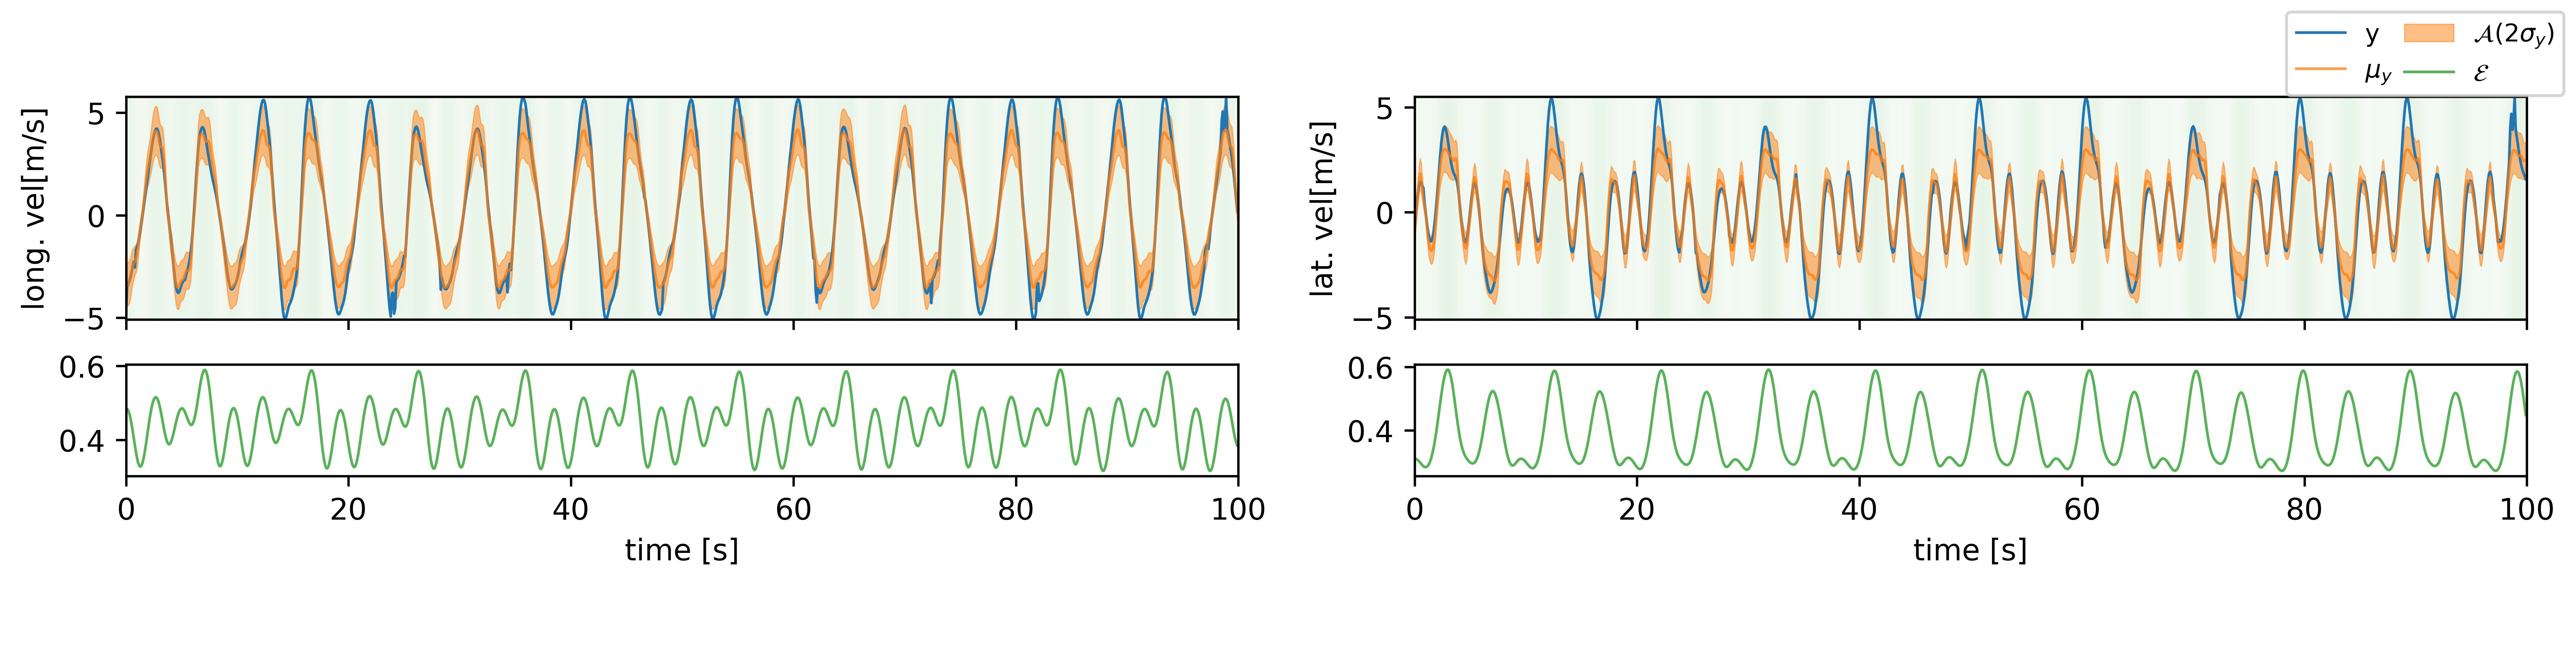
\includegraphics[width=\textwidth]{Experiments/figs/bb1_dropout_test.png}
%     \caption{Test}
%   \end{subfigure}
  
%   \begin{subfigure}[b]{\textwidth}
%     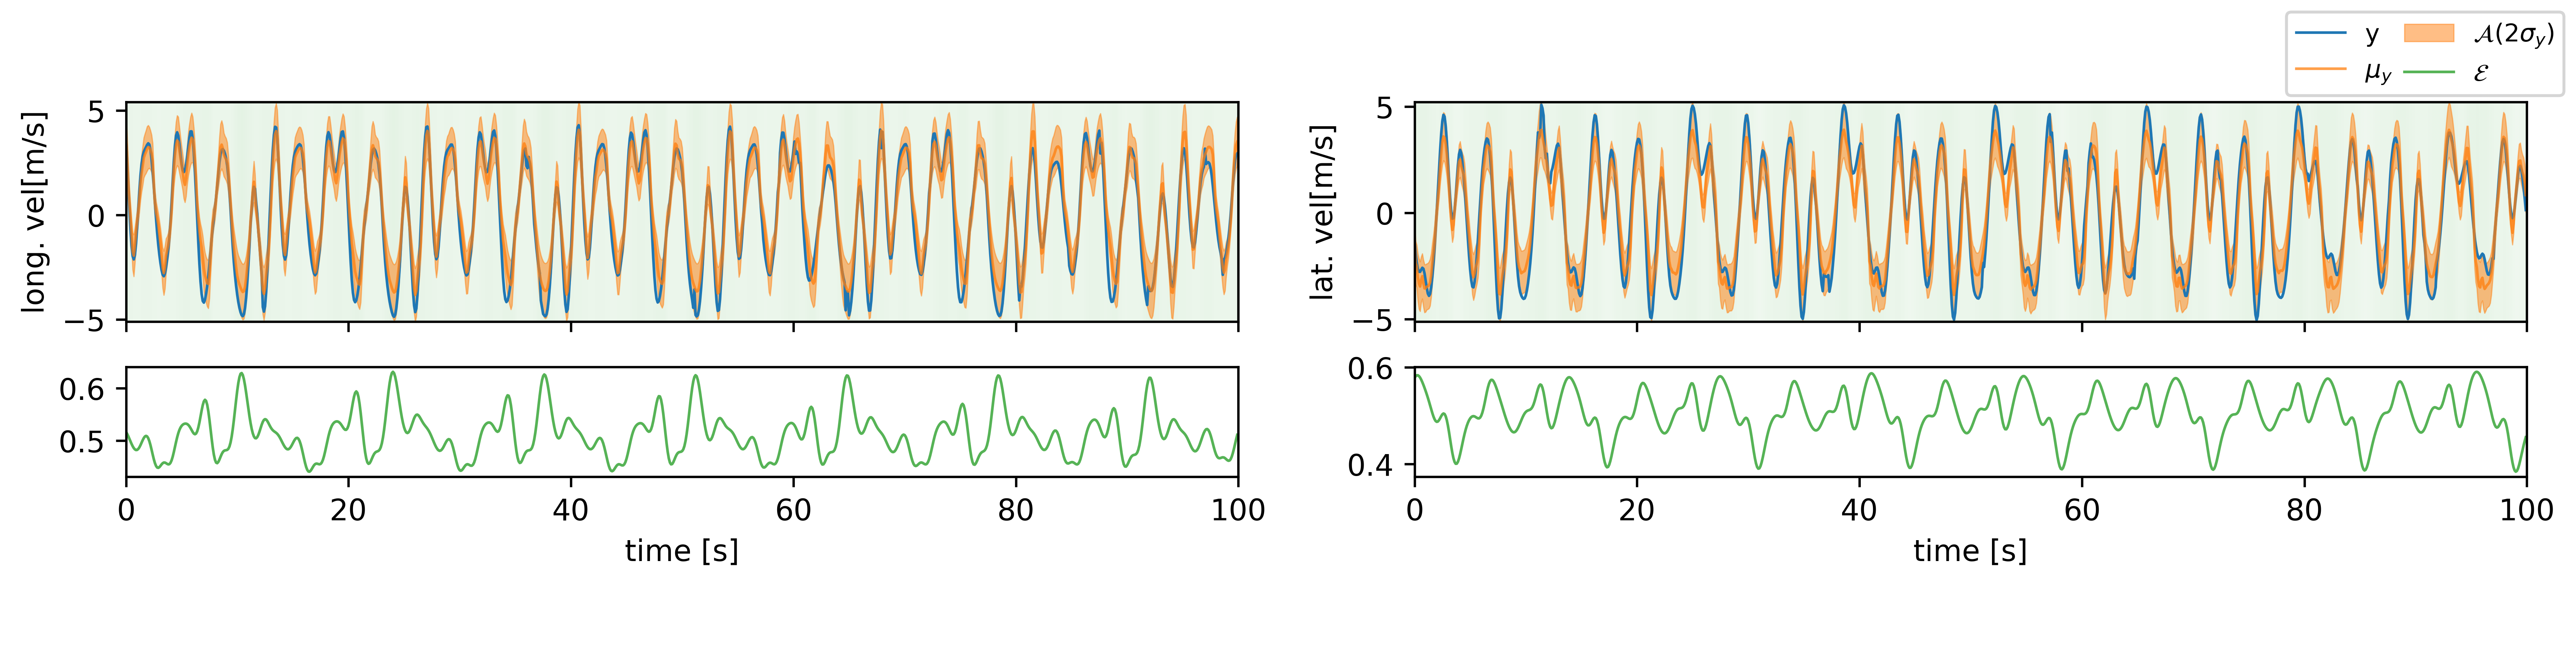
\includegraphics[width=\textwidth]{Experiments/figs/bb1_dropout_ood.png}
%     \caption{OOD}
%   \end{subfigure}
  
%   \caption{Blackbird(1) prediction plots for MC dropout.}
%   \label{fig:bb1_dropout_run}
% \end{figure}

\Cref{fig:bb1_dropout_run} shows a flight sequence with the model predictions for a test and an OOD sequence for the MC dropout model. Again we can see from the plots that the model behavior and quality of predictions is quite similar for the two sequences. \Cref{tbl:bb1_dropout} contains the basic performance metrics for the MC dropout model, and again we see that the model performance is similar for the test and OOD splits.

In terms of discriminating between the two splits, we can already see in \cref{tbl:bb1_dropout} that the uncertainties are on average the same for the test and OOD split. In fact the AUROC for MC dropout is 0.46 using the epistemic uncertainty. We show the correlation between the uncertainties and errors for MC dropout in \cref{tbl:bb1_dropout_corr} . We see similar trends to those of C-RNN in \cref{tbl:bb1_corr}, with both the aleatoric and epistemic uncertainties highly correlated with the MAE for all splits. Finally we compute the Pearson correlation between the epistemic and aleatoric uncertainties for the dropout model and get a 0.96 coefficient, showing that the uncertainties are also highly correlated for MC dropout. In the next subsection we will distill the key findings from the previous results and contrast the behavior of C-RNN and MC dropout in this setting.

\begin{table*}[ht]
\centering
    \begin{tabular}{l l c c c c}  
        \toprule
        U. & Split & \multicolumn{2}{c}{MAE} & \multicolumn{2}{c}{$Zs$}\\
        \midrule
        & & $\rho \uparrow$ & $r \uparrow$ & $\rho \uparrow$ & $r \uparrow$ \\
        \multirow{3}{*}{$\mathcal{A}$} 
            & Test     & 0.78(0.80, 0.76) & 0.82(0.82, 0.82) & - & - \\  
            & OOD      & 0.79(0.82, 0.75) & 0.85(0.85, 0.84) & - & - \\  
            & Test+OOD & 0.79(0.82, 0.76) & 0.83(0.84, 0.82) & - & - \\ 

        \midrule
        \multirow{3}{*}{$\mathcal{E}$} 
            & Test     & 0.76(0.76, 0.75) & 0.81(0.8, 0.81) &  0.42(0.42, 41)  & 0.45(0.43, 0.47) \\  
            & OOD      & 0.77(0.82, 0.72) & 0.83(0.84, 0.82) &  0.4(0.44, 0.35) & 0.45(0.49, 0.41) \\
            & Test+OOD & 0.76(0.79, 0.73) & 0.82(0.82, 0.81) &  0.4(0.43, 0.36) & 0.45(0.47, 0.42) \\ 

        \toprule
    \end{tabular}
    \caption[Blackbird(1) error-uncertainty correlations for MC dropout]{Blackbird(1) Pearson $\rho$ and Spearman $r$ correlations between the uncertainties and error scores for MC dropout.}
    \label{tbl:bb1_dropout_corr}
\end{table*}

\begin{figure}[htbp]
  \centering
    \begin{subfigure}[b]{\textwidth}
        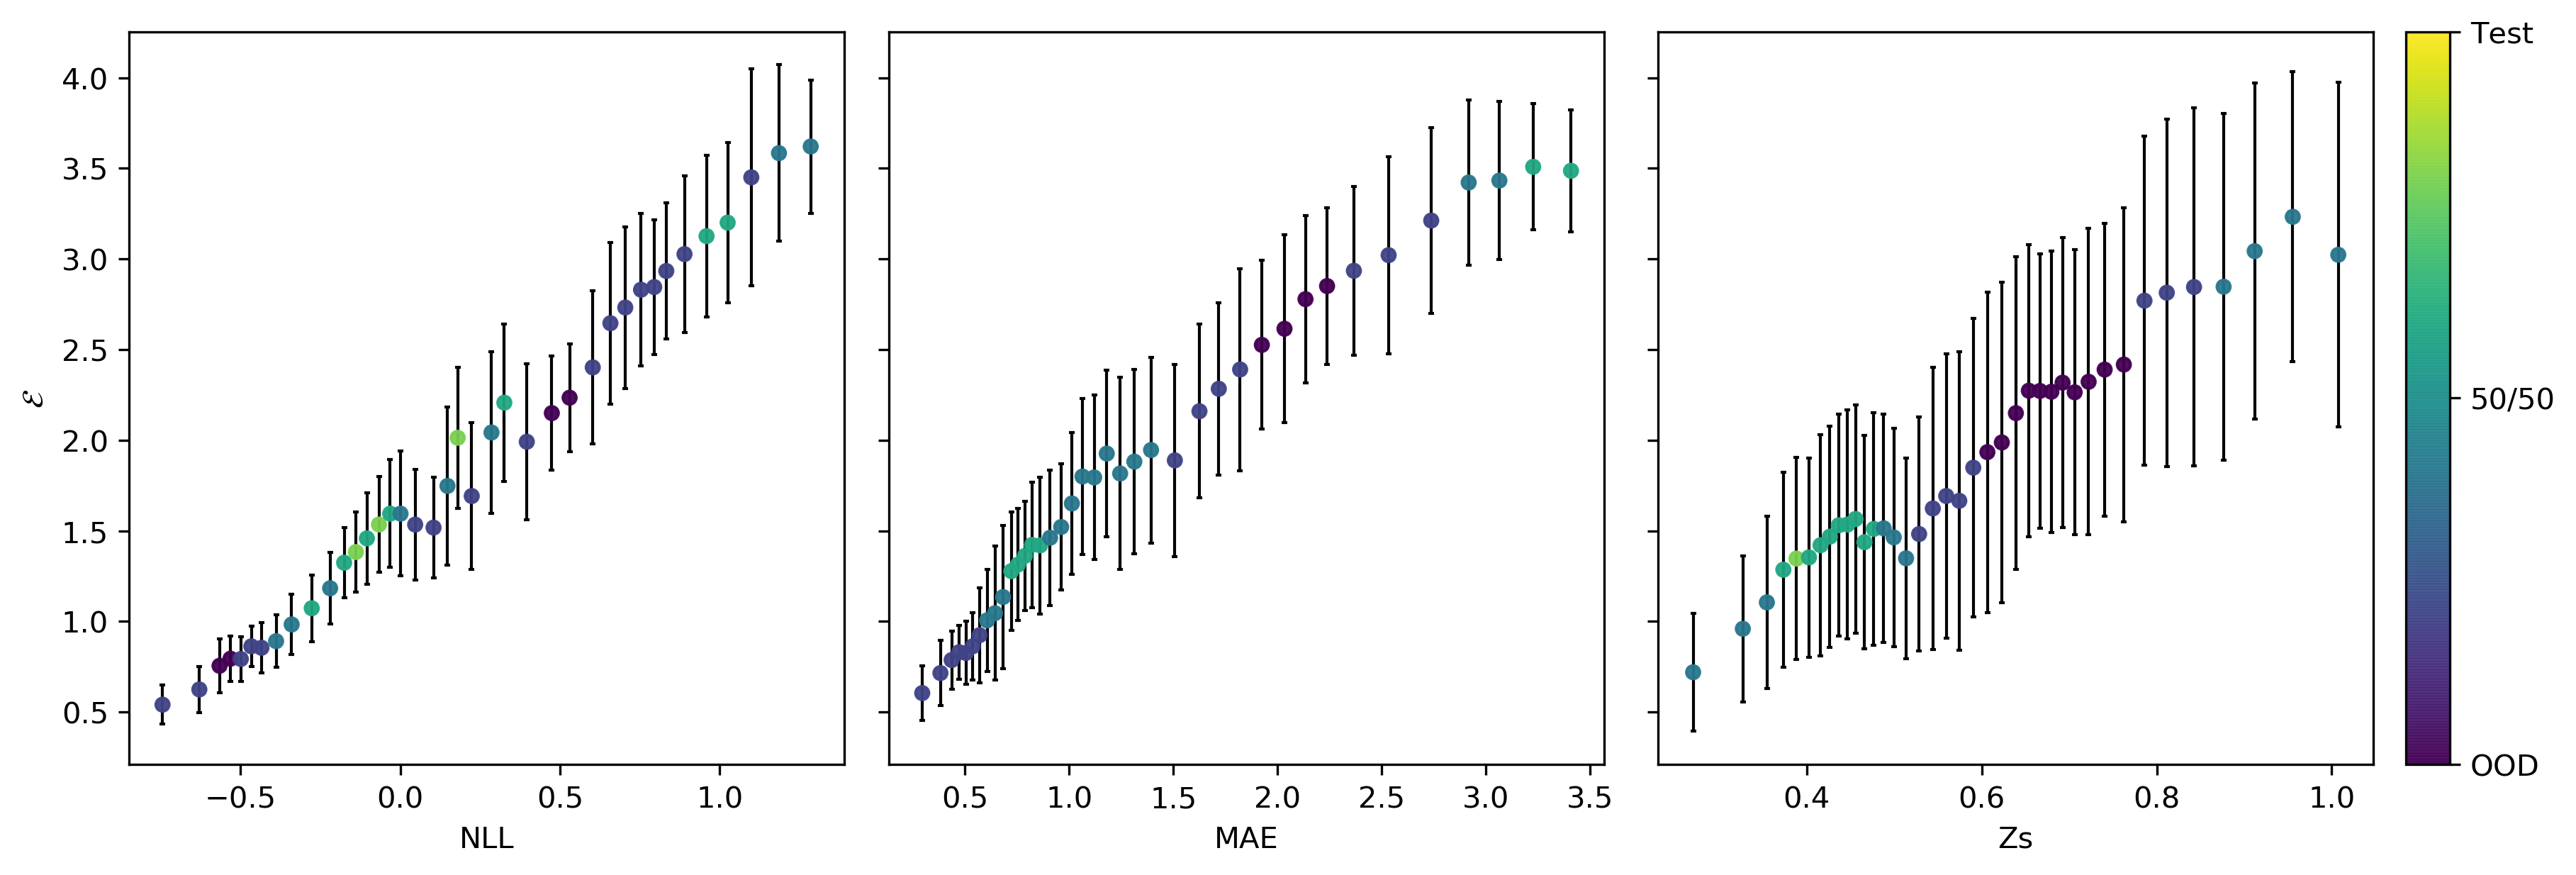
\includegraphics[width=\textwidth]{Experiments/figs/binned/bb1_dropout_epistemic.png}
        \caption{Binned diagonal plots for the epistemic uncertainty.}
    \end{subfigure}
    
    \begin{subfigure}[b]{\textwidth}
        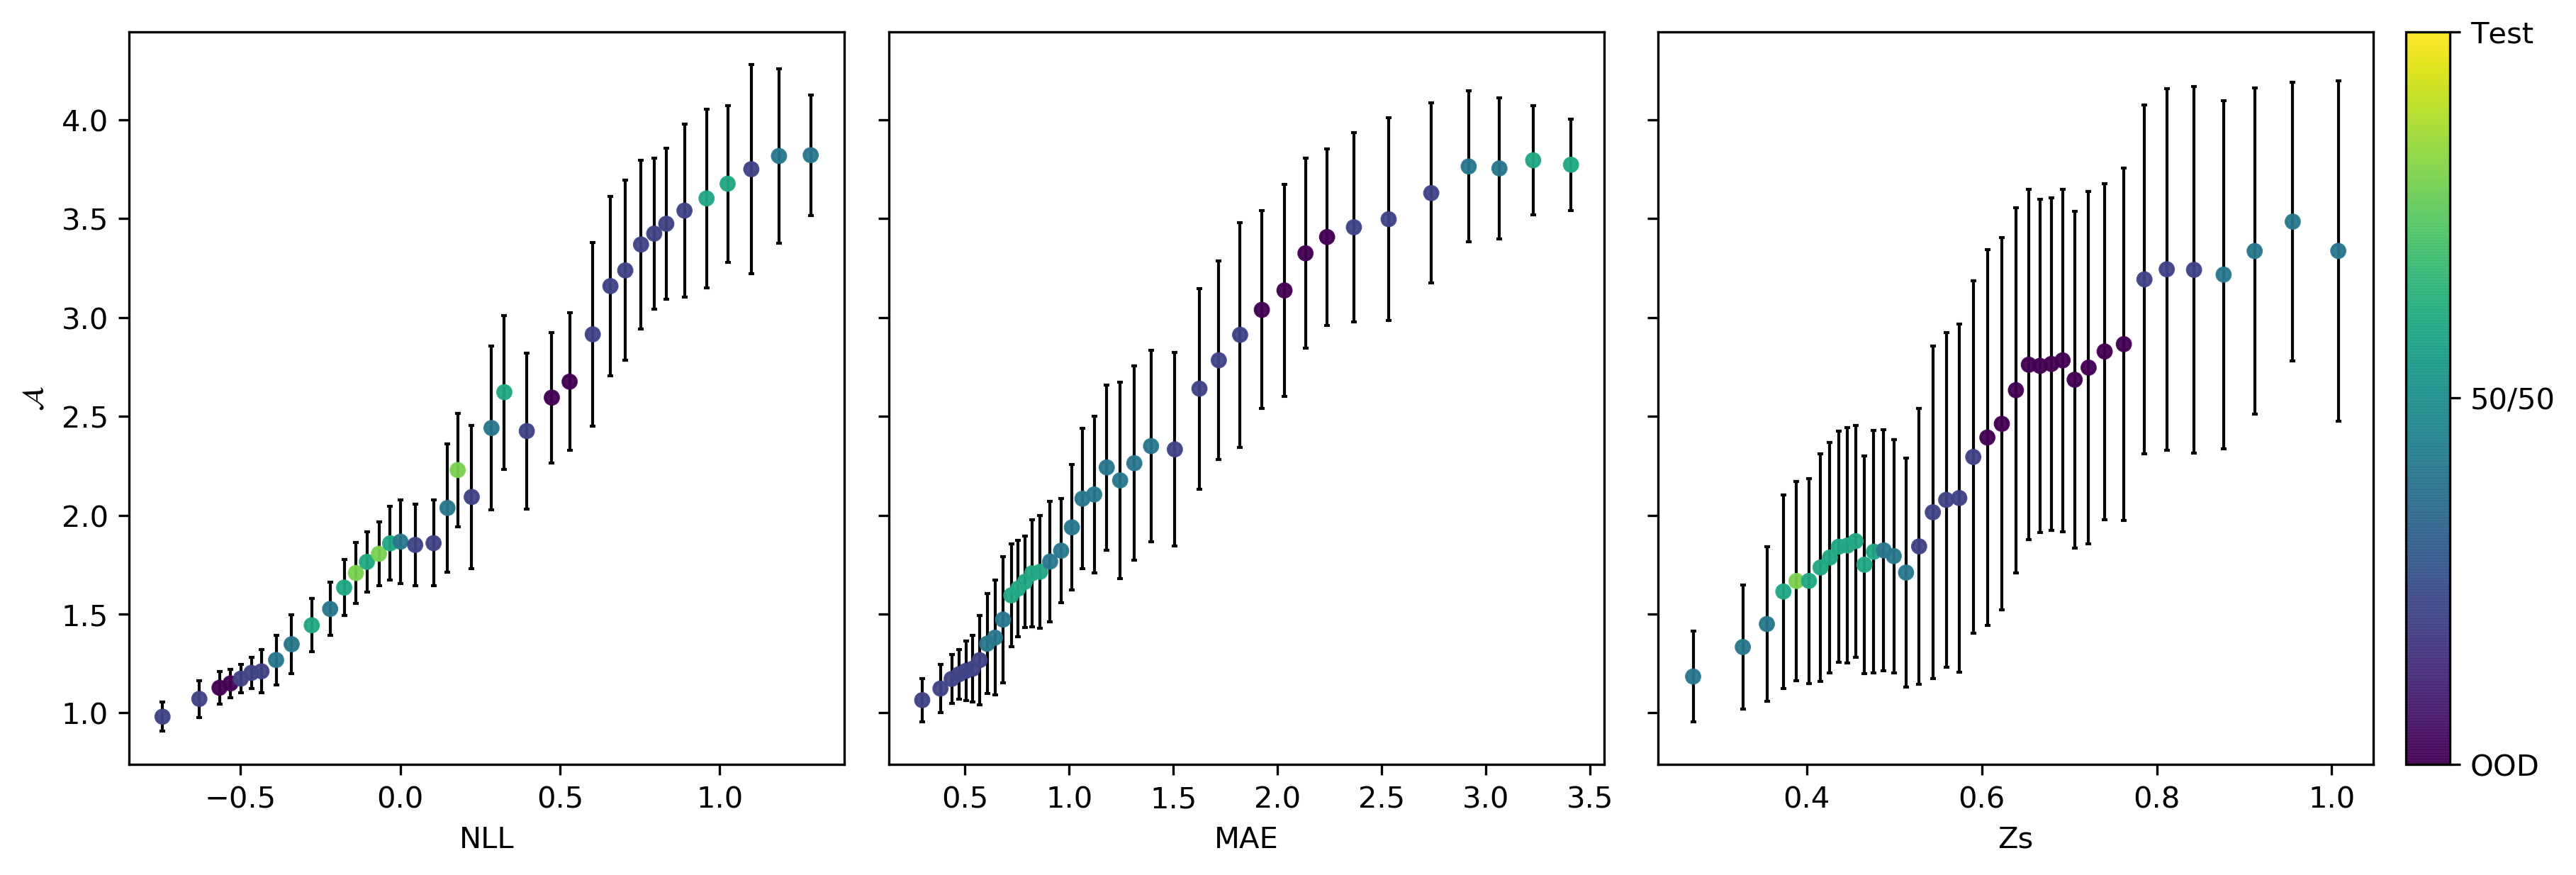
\includegraphics[width=\textwidth]{Experiments/figs/binned/bb1_dropout_aleatoric.png}
        \caption{Binned diagonal plots for the aleatoric uncertainty.}
  \end{subfigure}
    \caption[Blackbird(1) error-uncertainty diagonal plots for MC dropout]{Blackbird(1) binned diagonal plots of the  uncertainty vs error scores(NLL, MAE, Z-score) over the combined splits(Test+OOD). The marker color denotes the ratio of test to OOD points in the bin. }
    \label{fig:bb1_dropout_uncertainty_corr}
\end{figure}

\Cref{fig:bb1_dropout_uncertainty_corr} shows the binned diagonal plots for the errors versus uncertainty for MC dropout. The general patterns for the error-uncertainty correlations here are the same as for the C-RNN model. We see that both uncertainties behave similarly, the in/out-of-distribution points seem mixed within the bins, and both uncertainties correlate with the errors. 



\subsection{Key findings}

Recall that a key property of how we split the Blackbird dataset for this experiment was that the models could generalize to the OOD data. The key findings for our first split of Blackbird

\begin{itemize}
    \item Both models generalize well to the OOD data.
    \item Both models' epistemic uncertainty is on average equal for the test and OOD data.
    \item Both model show a high correlation between the MAE and the uncertainties.
    \item Both models a high correlation between their epistemic and aleatoric uncertainty estimates. 
\end{itemize}{}

In short, C-RNN and MC dropout qualitatively behave the same here. \Cref{tbl:bb1_comparison} shows the key results for both models. We can see that the performance of both models is close with the NLL being equal. For the epistemic uncertainty, we can see the C-RNN's epistemic uncertainty correlates slightly better with the MAE, giving a Pearson coefficient of 0.88 versus 0.76 for MC dropout. The correlation with the Z-score is roughly the same for both models. Also as we have mentioned both models show high correlation between their epistemic and aleatoric uncertainty estimate(C-RNN: 0.95, MC dropout: 0.96).  


\begin{table*}[h]
\centering
    \begin{tabular}{l l c c c c c}  
        \toprule
        Model & split & MAE & NLL & $\rho$(MAE vs $\mathcal{E}$) &
        $\rho$(Z-score vs $\mathcal{E}$) & AUROC($\mathcal{E}$)\\
        \midrule
        \multirow{3}{*}{C-RNN} 
            & Test     & 0.3  & 0.3  & 0.88  & 0.31 & - \\  
            & OOD      & 0.27 & 0.13 & 0.90  & 0.51 & -\\  
            & Test+OOD & 0.28 & 0.21 & 0.88  & 0.44 & 0.46\\ 

        \midrule
        \multirow{3}{*}{MC dropout} 
            & Test     & 0.26 & 0.2  & 0.76  & 0.42 & - \\  
            & OOD      & 0.28 & 0.23 & 0.77  & 0.4 & -\\  
            & Test+OOD & 0.27 & 0.21 & 0.76  & 0.4 & 0.46\\ 

        \toprule
    \end{tabular}
    \caption{Blackbird(1) key results for comparison of C-RNN and MC dropout.}
    \label{tbl:bb1_comparison}
\end{table*}


To conclude, we have created a situation where OOD inputs do not have higher errors than in-distribution inputs. This should be a challenging setting for C-RNN, as we have seen on the Revs dataset(\cref{sec:revs_results}), it consistently gave higher uncertainty to OOD inputs with an AUROC of 0.97. In this setting, this behavior would lead the epistemic uncertainty to be misleading. However, C-RNN handles the situation well, and preforms on par with MC dropout. In the coming section we will show a different set of experiments with the Blackbird dataset, where we chose a different in/out-of-distribution split. 


\clearpage
\section{Blackbird(2) results}

In the following set of experiments we will split Blackbird by yaw, meaning that sequences with constant yaw will be considered in-distribution and sequences with forward yaw will form the OOD split. This split, unlike the previous one, results in the models being unable to generalize well to the OOD data. This section will be structured like the previous one. We start with an analysis of C-RNN results, followed by MC dropout results, followed by key findings and comparison of the two models.

\subsection{C-RNN analysis}

\begin{figure}[h]
  \centering
  
  \begin{subfigure}[b]{\textwidth}
    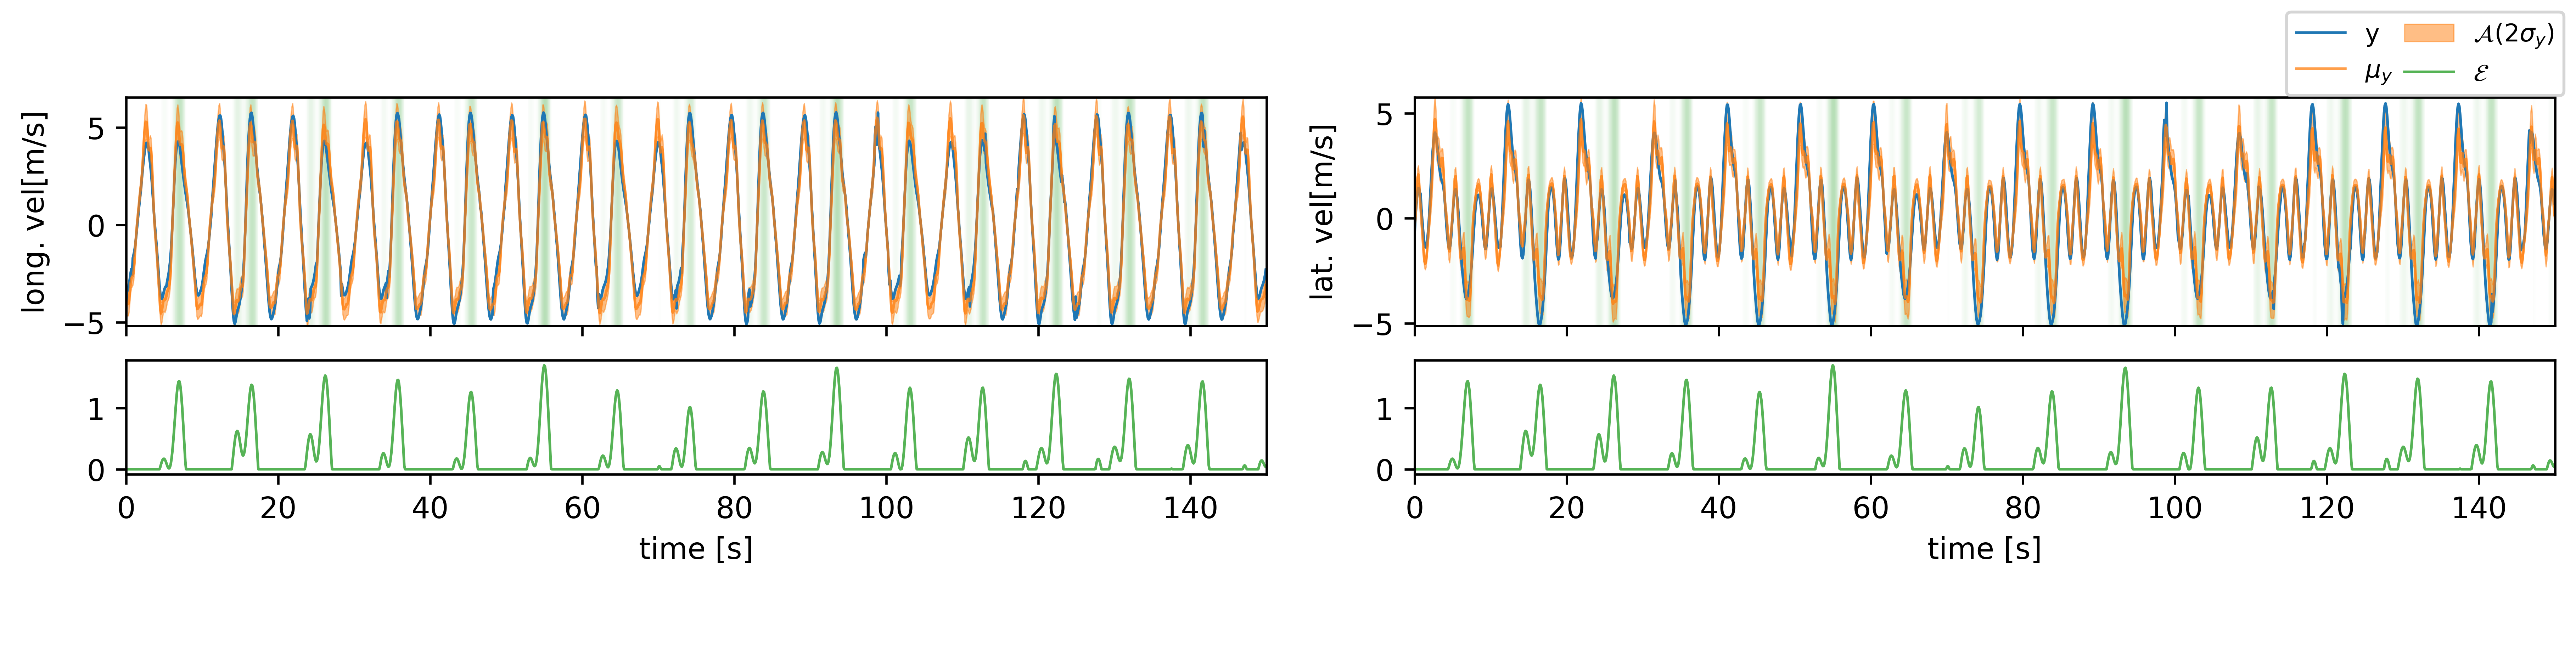
\includegraphics[width=\textwidth]{Experiments/figs/bb2_test.png}
    \caption{Test}
  \end{subfigure}
  
  \begin{subfigure}[b]{\textwidth}
    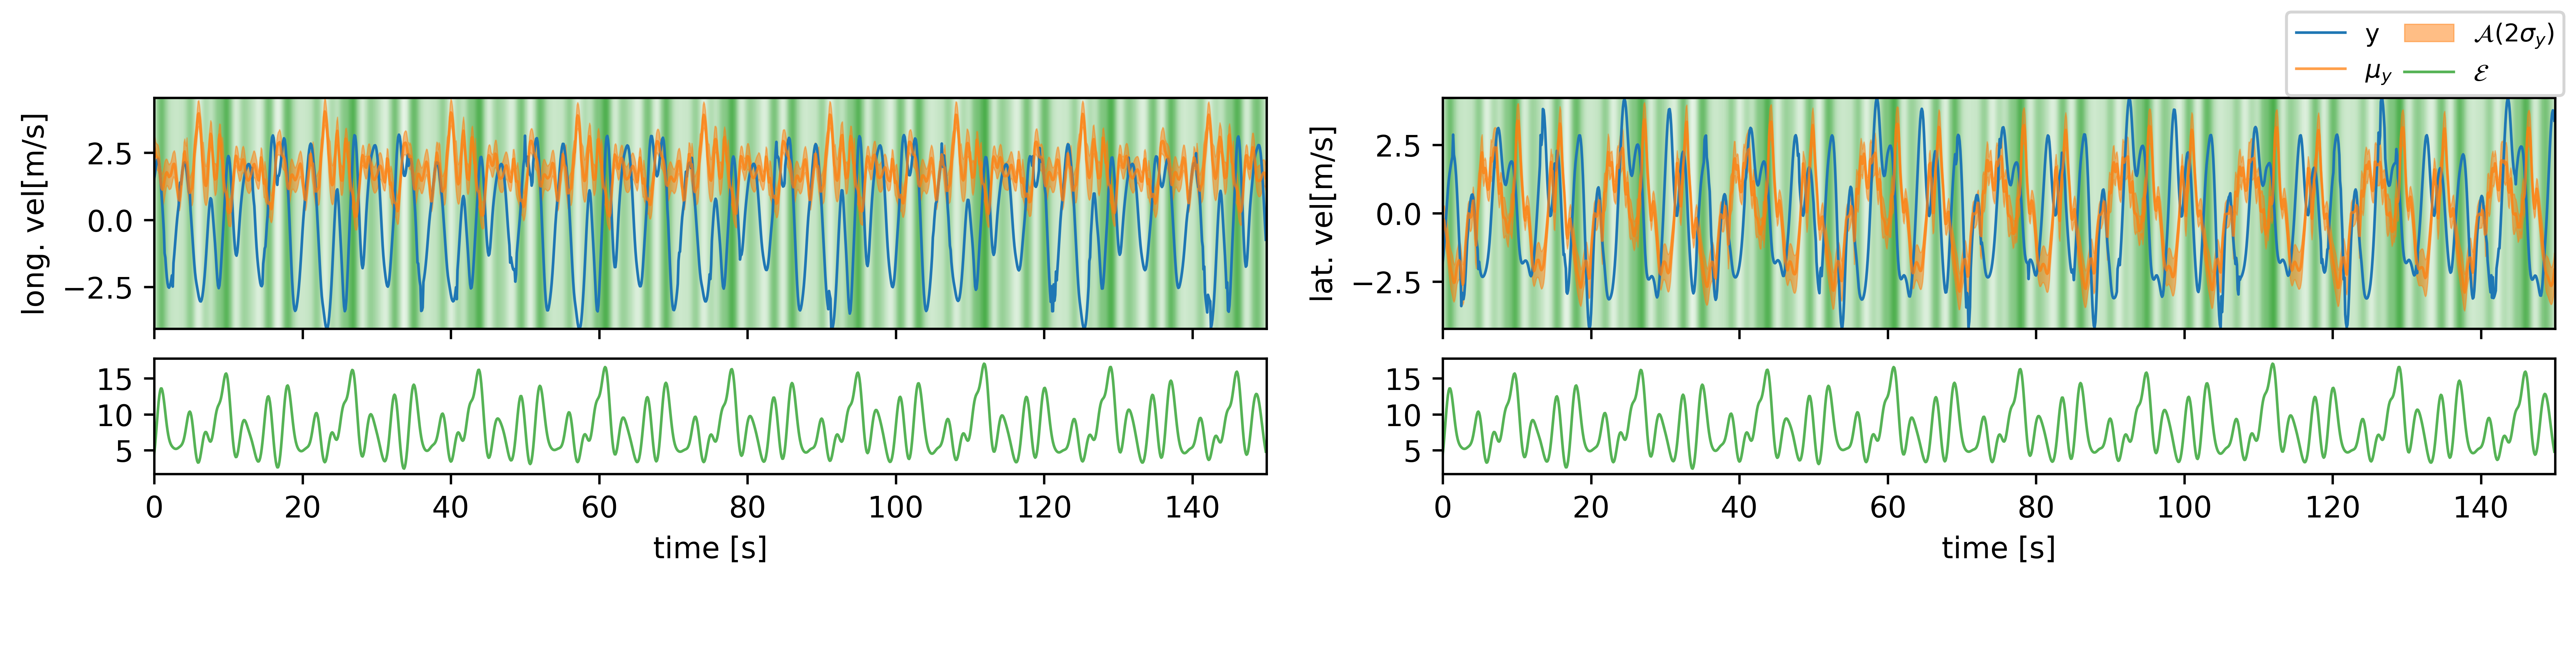
\includegraphics[width=\textwidth]{Experiments/figs/bb2_ood.png}
    \caption{OOD}
  \end{subfigure}
  
  \caption[Blackbird(2) prediction plots for C-RNN]{Blackbird(2) prediction plots for C-RNN. For plot description see \cref{sec:crnn_analysis}}
  \label{fig:bb2_run}
\end{figure}

\begin{table*}[h]
\centering
    \begin{tabular}{c  c  c   c  c }  
        \toprule
        Split & MAE & NLL & $\mathcal{A}$ & $\mathcal{E}$\\
        \midrule
        Test & 0.27(0.27, 0.32) & 0.22(0.14, 0.31) & 0.29(0.33, 0.33) &  -6.8\\
        OOD  &  1.12(1.2, 1) &  11.2(11.8, 10.6) & 0.35(0.6, 0.34)&  -3\\
        \midrule
    \end{tabular}
    \caption[Blackbird(2) C-RNN performance]{Blackbird(2) C-RNN performance.}
    \label{tbl:bb2_CRNN}
\end{table*}


\cref{fig:bb2_run} shows a flight sequence with the model predictions for a test and an OOD input. We can see from the plots that the model performs significantly worse on the OOD sequence. The epistemic uncertainty is much higher on the OOD input. \Cref{tbl:bb2_CRNN} shows the basic perfomance results. We the MAE for the test split is 0.27, and for the OOD split it is 1.15. The NLL of the test split is 0.22, for the OOD split it is 11.2. Thus the numbers show a significant decrease in performance between the splits. The average aleatoric uncertainty for the test split is 0.29, for the OOD split is 0.35. This already suggests that the aleatoric uncertainty does capture the increase in errors the model sees over the OOD data. The average epistemic uncertainty however goes from -6.8 over the test split, to -3 over the OOD split. This gives hope that the epistemic uncertainty captures the large errors the model commits for OOD inputs. 

\begin{table*}[h]
\centering
    \begin{tabular}{c  c  c}  
        \toprule
        Uncertainty score & AUROC$\uparrow$ & FPR@95\%$\downarrow$\\
        \midrule
        Aleatoric($\mathcal{A}$) & 0.54  & 0.8\\
        Epistemic($\mathcal{E}$) & 0.8 &  0.56 \\
        \midrule
    \end{tabular}
    \caption{Blackbird(2) OOD discrimination power for MC dropout.}
    \label{tbl:bb2_discrimination}
\end{table*}

\Cref{tbl:bb2_discrimination} shows how well our uncertainties can discriminate between the two splits. We can see that the aleatoric uncertainty does slightly better than random with an AUROC of 0.54. The epistemic uncertainty has a better AUROC of 0.8, which means a random OOD input has probability 0.8 of having higher epistemic uncertainty than a test input. 

It is challenging to gauge how good or bad the AUROC of 0.8 is in this context. Again, to better judge the quality of the uncertainty estimates we look at the correlation between the uncertainties and the errors. \Cref{tbl:bb2_corr} show the correlations between our uncertainties and error scores. First we note that the aleatoric uncertainty correlates very well with the MAE on each split individually, with a roughly 0.9 Pearson correlation with the MAE for both the test and OOD splits individually. However, over the combined split, we see that the aleatoric uncertainty gives a weaker correlation of 0.7. This makes sense given the aleatoric uncertainty is on average the same for the test and OOD splits, while the MAE is more than four times larger over the OOD split. The epistemic uncertainty shows a strong correlation with the MAE over the individual splits and the combined split, with a Pearson correlation of 0.9 over the combined splits. Moreover, we also see a strong Pearson correlation of 0.83 with the Z-score over the combined splits, suggesting that the epistemic uncertainty does go up for errors which are not explained away by the epistemic uncertainty. 


\begin{table*}[h]
\centering
    \begin{tabular}{l l c c c c}  
        \toprule
        U. & Split & \multicolumn{2}{c}{MAE} & \multicolumn{2}{c}{$Zs$}\\
        \midrule
        & & $\rho \uparrow$ & $r \uparrow$ & $\rho \uparrow$ & $r \uparrow$ \\
        \multirow{3}{*}{$\mathcal{A}$} 
            & Test     & 0.9(0.92, 0.87) & 0.89(0.89, 0.89) & - & - \\  
            & OOD      & 0.91(0.92, 0.89) & 0.94(0.94, 0.93) & - & - \\  
            & Test+OOD & 0.7(0.7, 0.7) & 0.74(0.72, 0.76) & - & - \\ 

        \midrule
        \multirow{3}{*}{$\mathcal{E}$} 
            & Test     & 0.92  & 0.91 &  0.48  & 0.63 \\  
            & OOD      & 0.87 & 0.91 &  0.83 & 0.83 \\
            & Test+OOD & 0.90 & 0.91 &  0.83 & 0.79 \\ 

        \toprule
    \end{tabular}
    \caption[Blackbird(2) error-uncertainty correlation for C-RNN]{Blackbird(2) error-uncertainty correlation for C-RNN. For table description see \cref{sec:crnn_analysis}}
    \label{tbl:bb2_corr}
\end{table*}


The correlation between the epistemic and aleatoric uncertainty is 0.61, suggesting that there is some overlap in the information they capture. But the results from \cref{tbl:bb2_corr} and \cref{tbl:bb2_discrimination} show that the epistemic uncertainty provides some information that is not contained in the aleatoric uncertainty. Namely, distinguishing between the in/out-of-distribution inputs. Next we will evaluate the performance of MC dropout. 

\begin{figure}[htbp]
  \centering
    \begin{subfigure}[b]{\textwidth}
        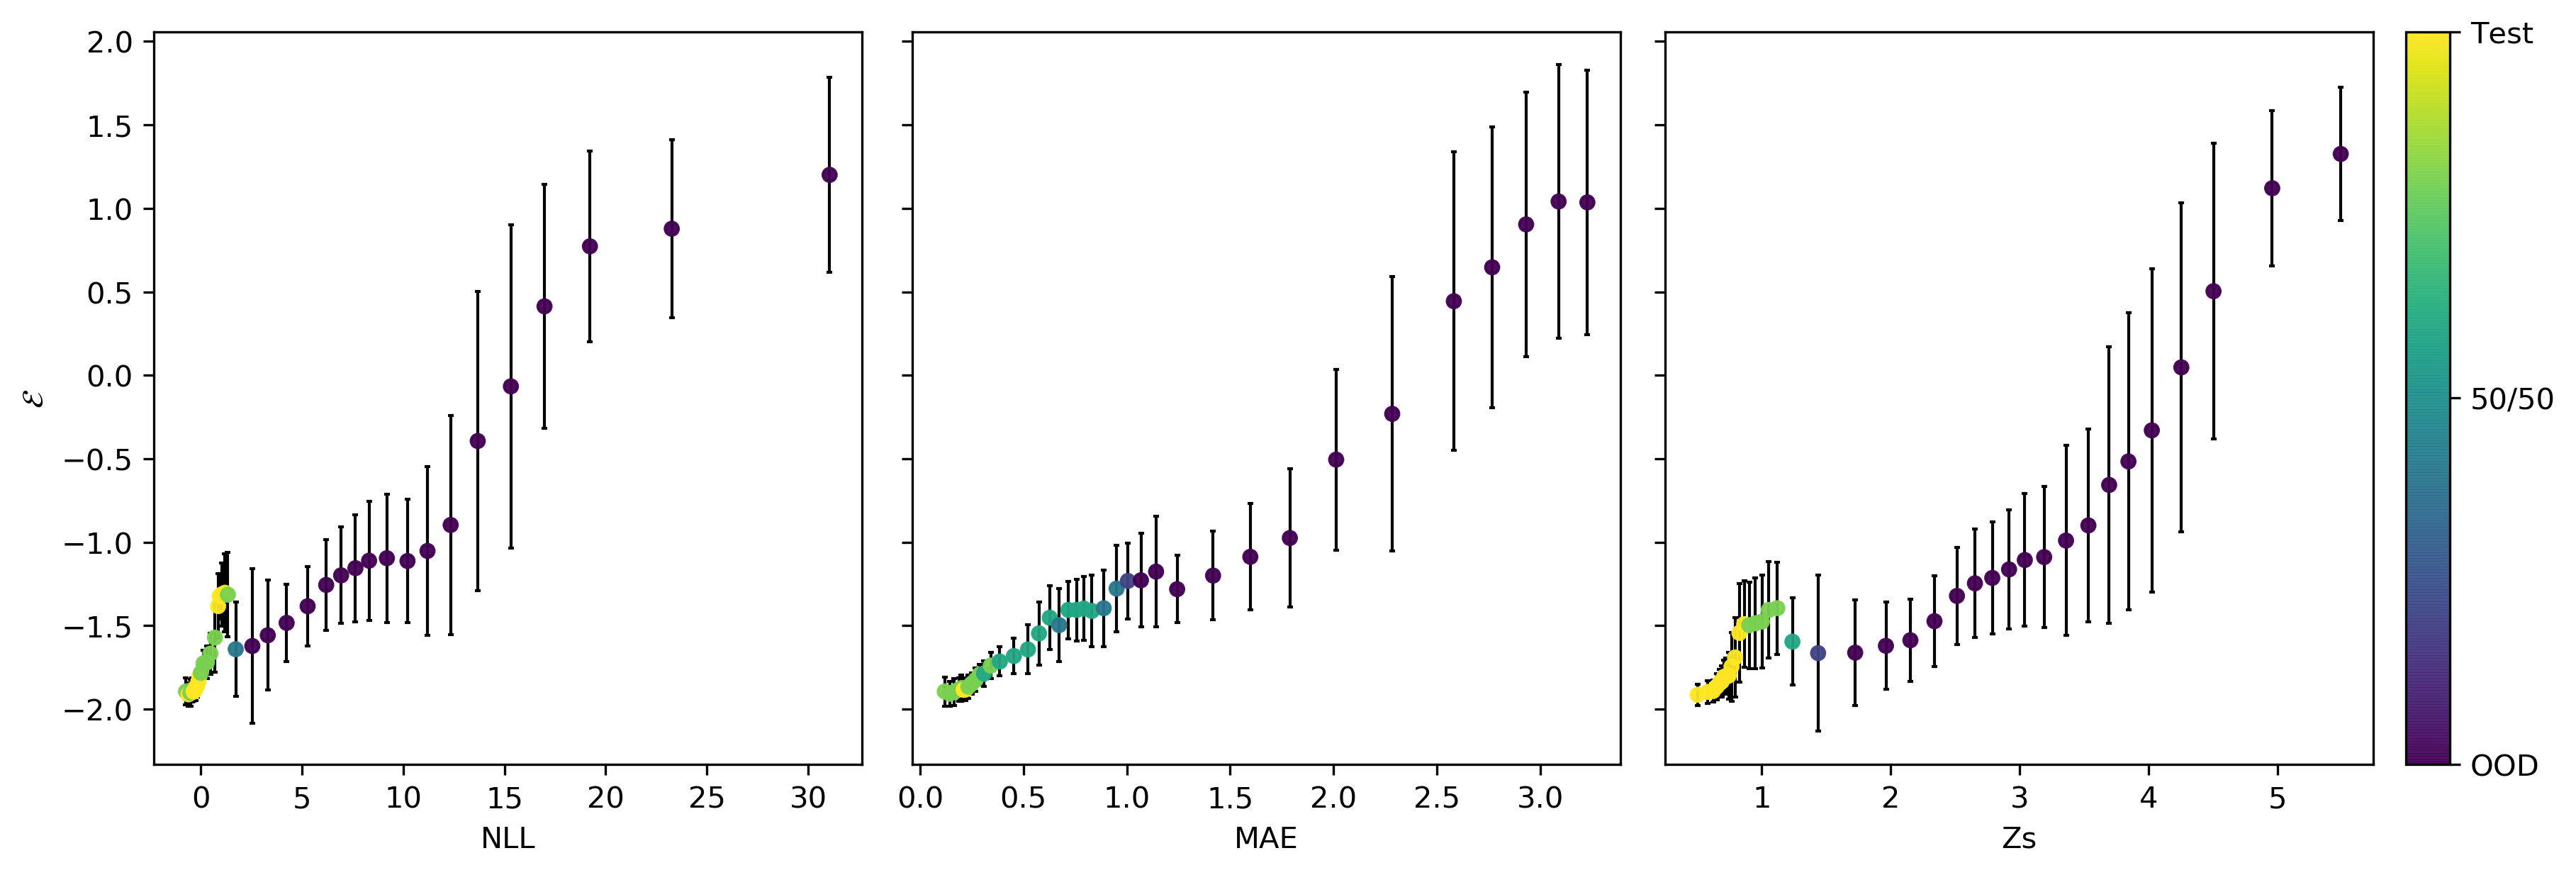
\includegraphics[width=\textwidth]{Experiments/figs/binned/bb2_crnn_epistemic.png}
        \caption{Binned diagonal plots for the epistemic uncertainty.}
    \end{subfigure}
    
    \begin{subfigure}[b]{\textwidth}
        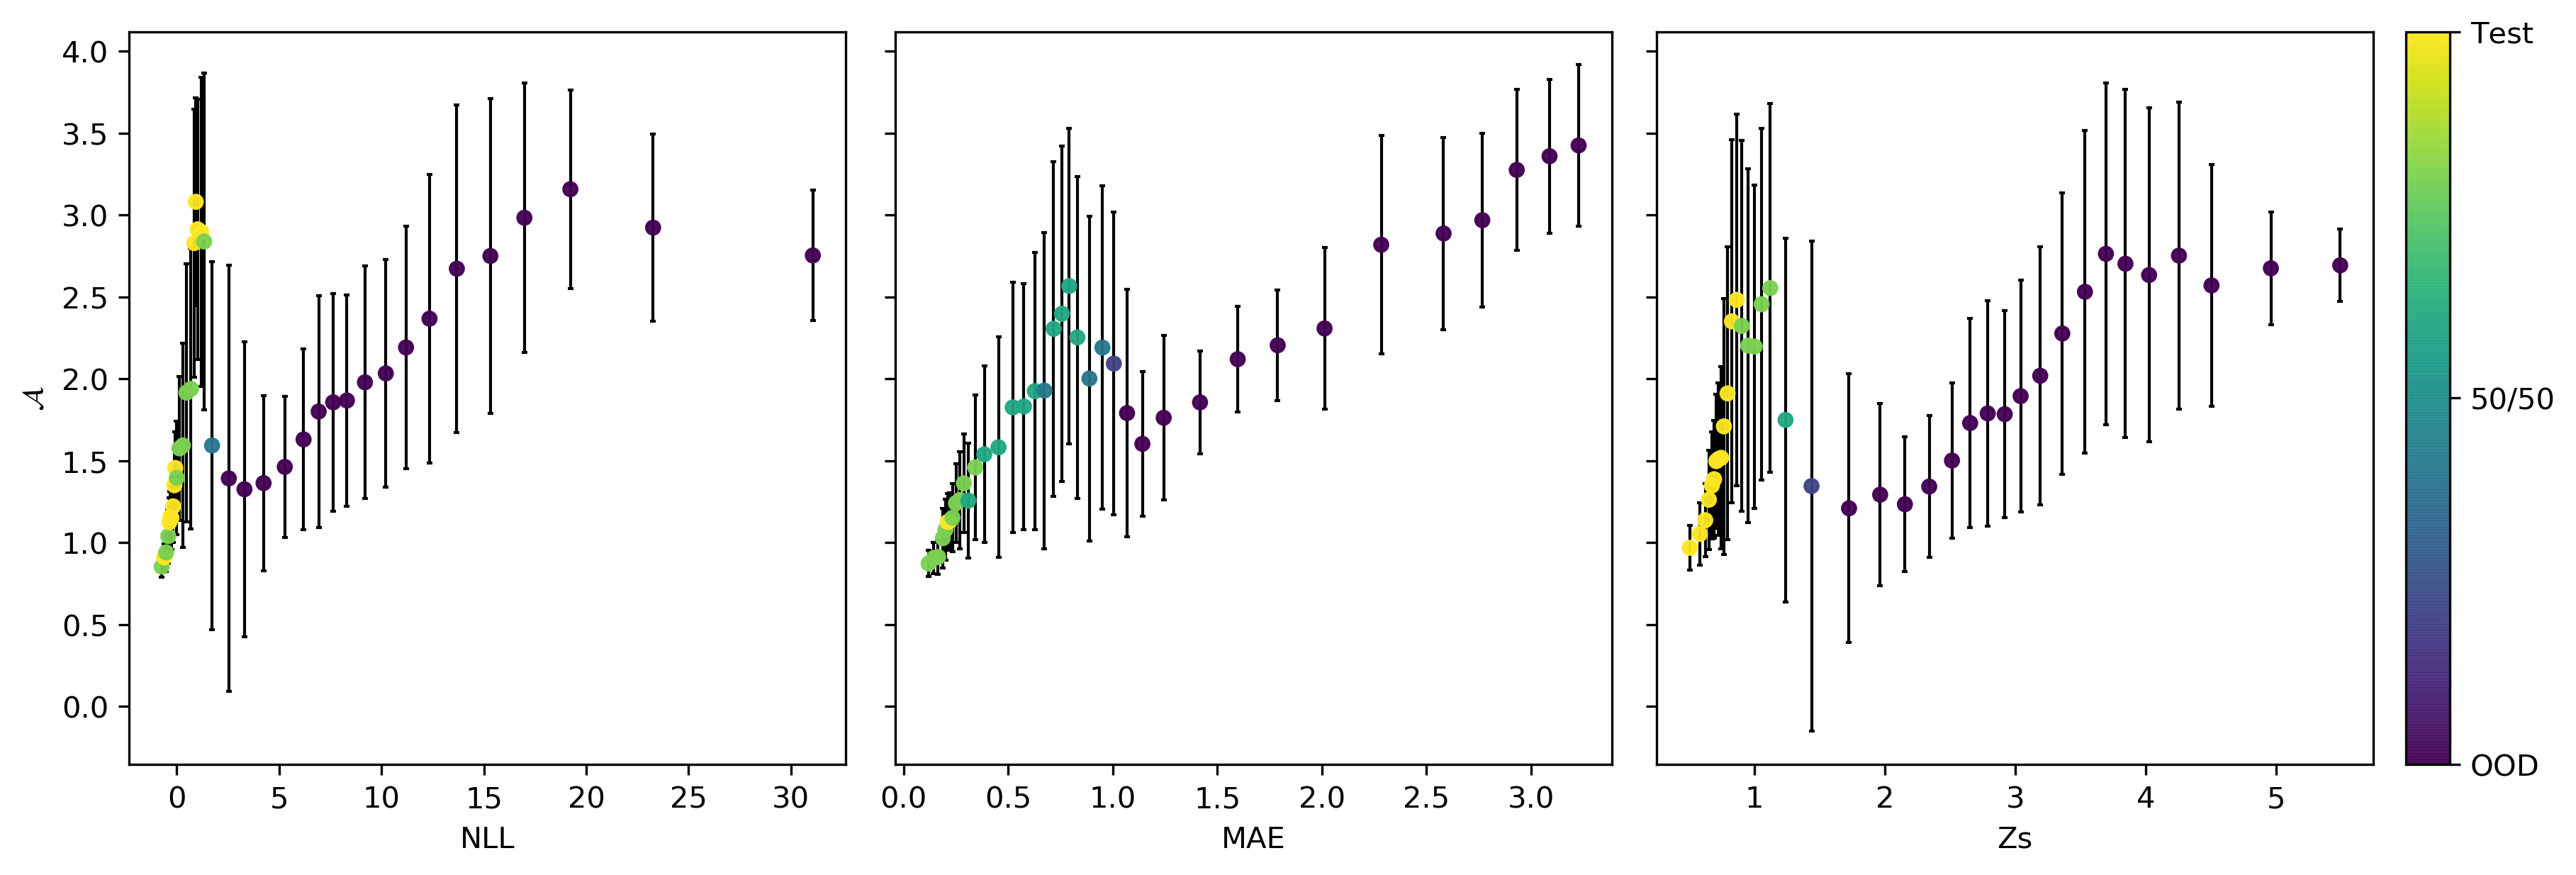
\includegraphics[width=\textwidth]{Experiments/figs/binned/bb2_crnn_aleatoric.png}
        \caption{Binned diagonal plots for the aleatoric uncertainty.}
  \end{subfigure}
    \caption[Blackbird(2) error-uncertainty diagonal plots for C-RNN]{Blackbird(2) error-uncertainty diagonal plots for C-RNN. For plot description see \cref{sec:crnn_analysis}}
    \label{fig:bb2_uncertainty_corr}
\end{figure}

\Cref{fig:bb2_uncertainty_corr} show the binned diagonal plots for errors versus uncertainties. The plots show that this split of Blackbird presents mixed results. Like the Revs results for C-RNN (\cref{fig:revs_uncertainty_corr}), the data seems to separated to a low error in distribution cluster, followed by a high error OOD tail. However, the pattern is not as clear.
Some of the bins in the two extremes seem to be mostly coming from a single split, but in the middle we see mixed bins. 
The aleatoric uncertainty exhibits the same dynamic we have seen on the Revs dataset(\cref{fig:revs_uncertainty_corr}), where it correlates well with the MAE in the beginning, then \emph{restarts} and correlates separately with the high error points. However, the pattern is not as strong here. 
The epistemic uncertainty correlates well with the errors and separates the in/out-of-distribution points, however not as strongly as we see on the Revs dataset. In the next section, we will see how dropout handles this case. 


\clearpage
\subsection{MC dropout analysis}

\begin{figure}[h]
  \centering
  
  \begin{subfigure}[b]{\textwidth}
    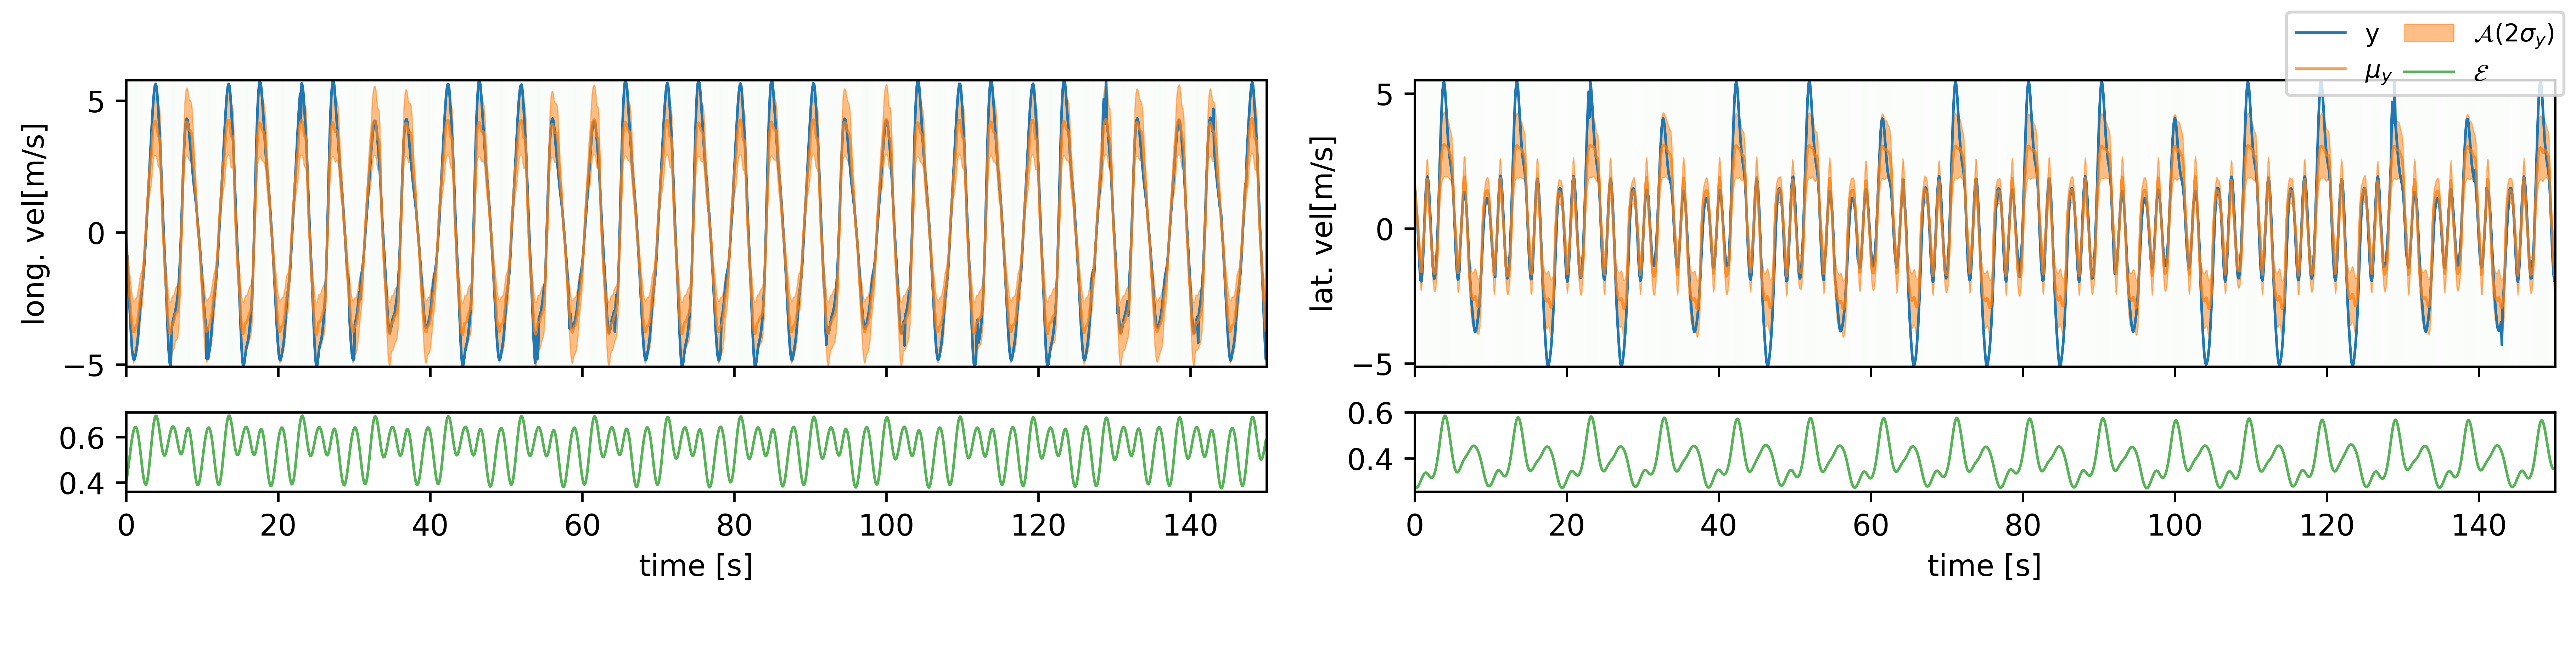
\includegraphics[width=\textwidth]{Experiments/figs/bb2_dropout_test.png}
    \caption{Test}
  \end{subfigure}
  
  \begin{subfigure}[b]{\textwidth}
    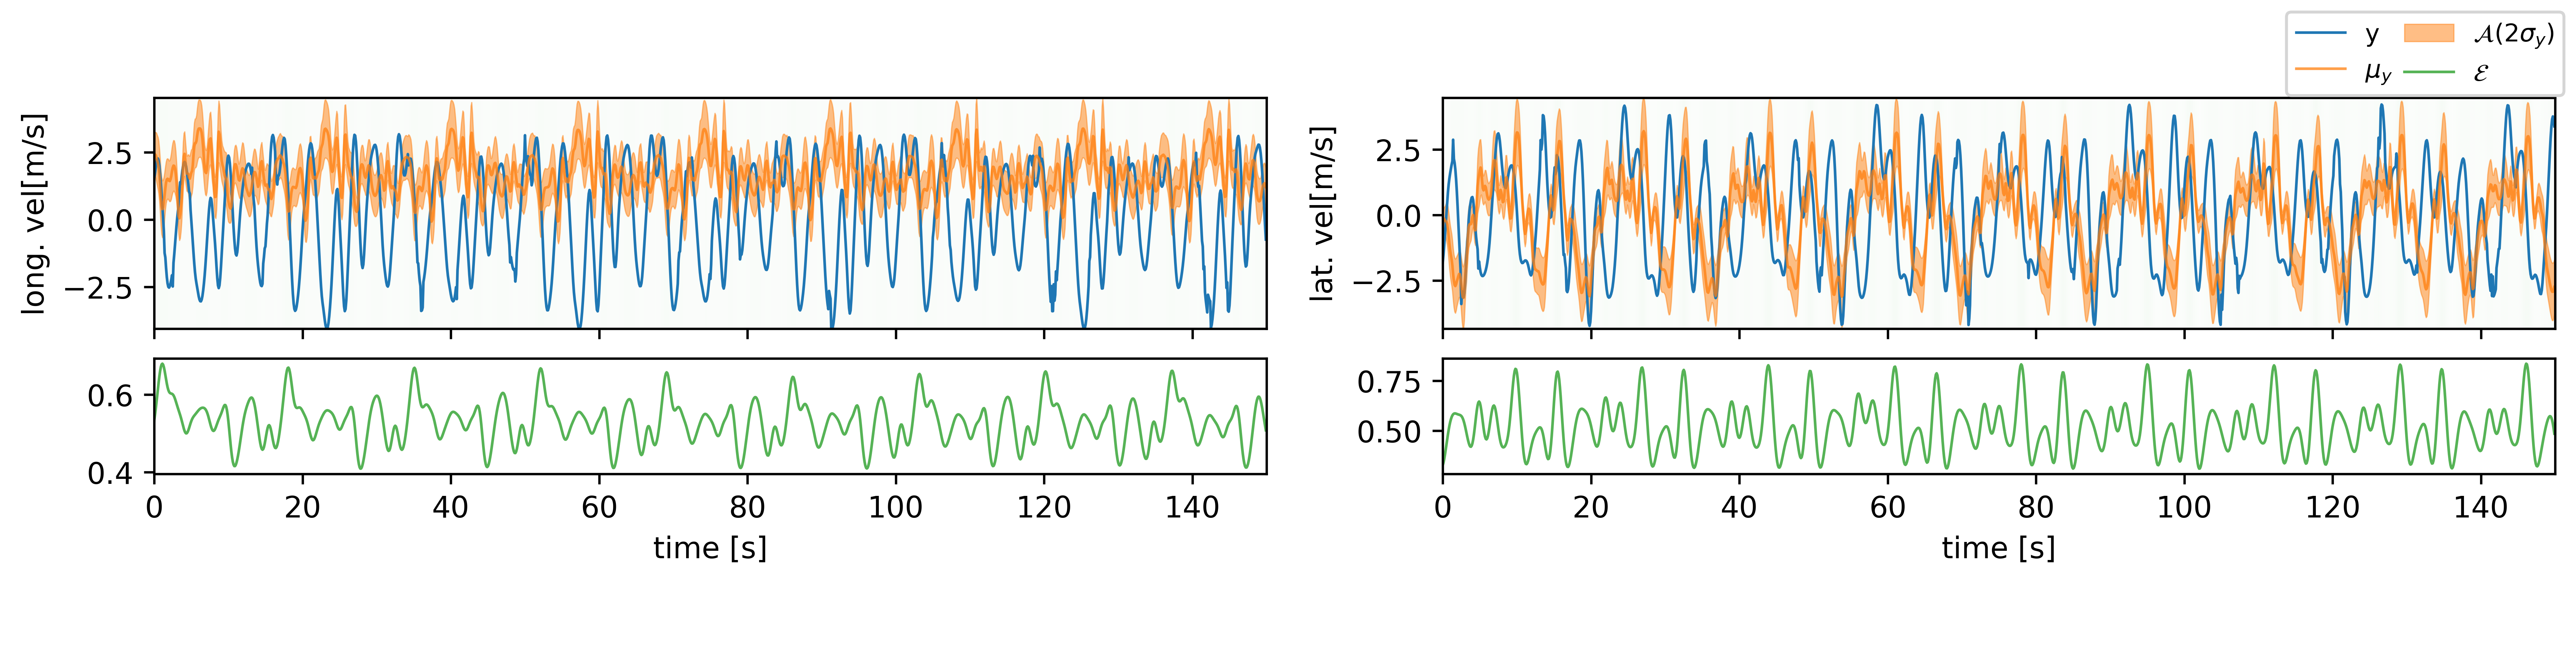
\includegraphics[width=\textwidth]{Experiments/figs/bb2_dropout_ood.png}
    \caption{OOD}
  \end{subfigure}
  
  \caption[Blackbird(2) prediction plots for MC dropout]{Blackbird(2) prediction plots for MC dropout. For plot description see \cref{sec:crnn_analysis}}
  \label{fig:bb2_dropout_run}
\end{figure}

\begin{table*}[h]
\centering
    \begin{tabular}{c  c  c  c  c }  
        \toprule
        Split & MAE & NLL & $\mathcal{A}$ & $\mathcal{E}$\\
        \midrule
        Test & 0.27(0.26, 0.29) & 0.22(0.19, 0.25) & 0.42(0.42, 0.41) &  0.28(0.28, 0.28)\\
        OOD  &  1.1(1.14, 1) &  7.3(7.3, 7.4) & 0.33(0.35, 0.32)&  0.28(0.3, 0.26)\\
        \midrule
    \end{tabular}
    \caption{Blackbird(2) MC dropout performance.}
    \label{tbl:bb2_dropout}
\end{table*}



\Cref{fig:bb2_dropout_run} shows a flight sequence with the model predictions for a test and an OOD sequence for the MC dropout model. A familiar patter emerges, the model visibly performs worse on the OOD sample, yet the epistemic and aleatoric uncertainties don't seem to capture that decrease in accuracy. \Cref{tbl:bb2_dropout} contains the performance measures. We can see the MAE and NLL increase from 0.27 and 0.22 respectively over the test split, to 1.1 and 7.3 over the OOD split. However, the epistemic and aleatoric uncertainties show no increase with the aleatoric uncertainty being actually lower on the OOD split. \Cref{tbl:bb2_dropout_discrimination} confirms that neither the epistemic or aleatoric uncertainty from MC dropout provides a useful signal for detecting OOD inputs, with AUROC scores around 0.5 similar to the expected performance of a random classifier. 


\begin{table*}[h]
\centering
    \begin{tabular}{c  c  c}  
        \toprule
        Uncertainty score & AUROC$\uparrow$ & FPR@95\%$\downarrow$\\
        \midrule
        Aleatoric($\mathcal{A}$) & 0.48  & 0.82\\
        Epistemic($\mathcal{E}$) & 0.48 &  0.81 \\
        \midrule
    \end{tabular}
    \caption{blackbird(2) OOD discrimination power for MC dropout.}
    \label{tbl:bb2_dropout_discrimination}
\end{table*}

\Cref{tbl:bb2_dropout_corr} shows the correlations between the uncertainties and the errors for MC dropout. We see that both uncertainties show strong correlation with the MAE for the individual splits, but not for the combined split. The epistemic uncertainty only correlates weakly with the Z-score. Moreover, note that the performance of both uncertainties is very similar overall. 


\begin{table*}[h]
\centering
    \begin{tabular}{l l c c c c}  
        \toprule
        U. & Split & \multicolumn{2}{c}{MAE} & \multicolumn{2}{c}{$Zs$}\\
        \midrule
        & & $\rho \uparrow$ & $r \uparrow$ & $\rho \uparrow$ & $r \uparrow$ \\
        \multirow{3}{*}{$\mathcal{A}$} 
            & Test     & 0.84(0.88, 0.8) & 0.89(0.89, 0.88) & - & - \\  
            & OOD      & 0.89(0.94, 0.85) & 0.91(0.92, 0.9) & - & - \\  
            & Test+OOD & 0.49(0.51, 0.46) & 0.49(0.51, 0.47) & - & - \\ 

        \midrule
        \multirow{3}{*}{$\mathcal{E}$} 
            & Test     & 0.84(0.87, 0.8)  & 0.87(0.87, 0.87) & 0.43(0.42, 0.44) & 0.45(0.43, 0.46) \\  
            & OOD      & 0.91(0.93, 0.88) & 0.92(0.93, 0.91) & 0.54(0.67, 0.41) & 0.58(0.67, 0.5) \\
            & Test+OOD & 0.69(0.72, 0.65) & 0.69(0.72, 0.65) & 0.31(0.41, 0.2) & 0.3(0.39, 0.21) \\ 

        \toprule
    \end{tabular}
    \caption[Blackbird(2) error-uncertainty correlation for MC dropout]{Blackbird(2) error-uncertainty correlation for MC dropout. For table description see \cref{sec:crnn_analysis}}
    \label{tbl:bb2_dropout_corr}
\end{table*}

We compute the correlation between the aleatoric and epistemic uncertainty and obtain a Pearson coefficient of 0.94. This shows that for MC dropout both uncertainties give us mostly the same information. Again this was also found empirically by \cite{kendall2017uncertainties}. 

\begin{figure}[htbp]
  \centering
    \begin{subfigure}[b]{\textwidth}
        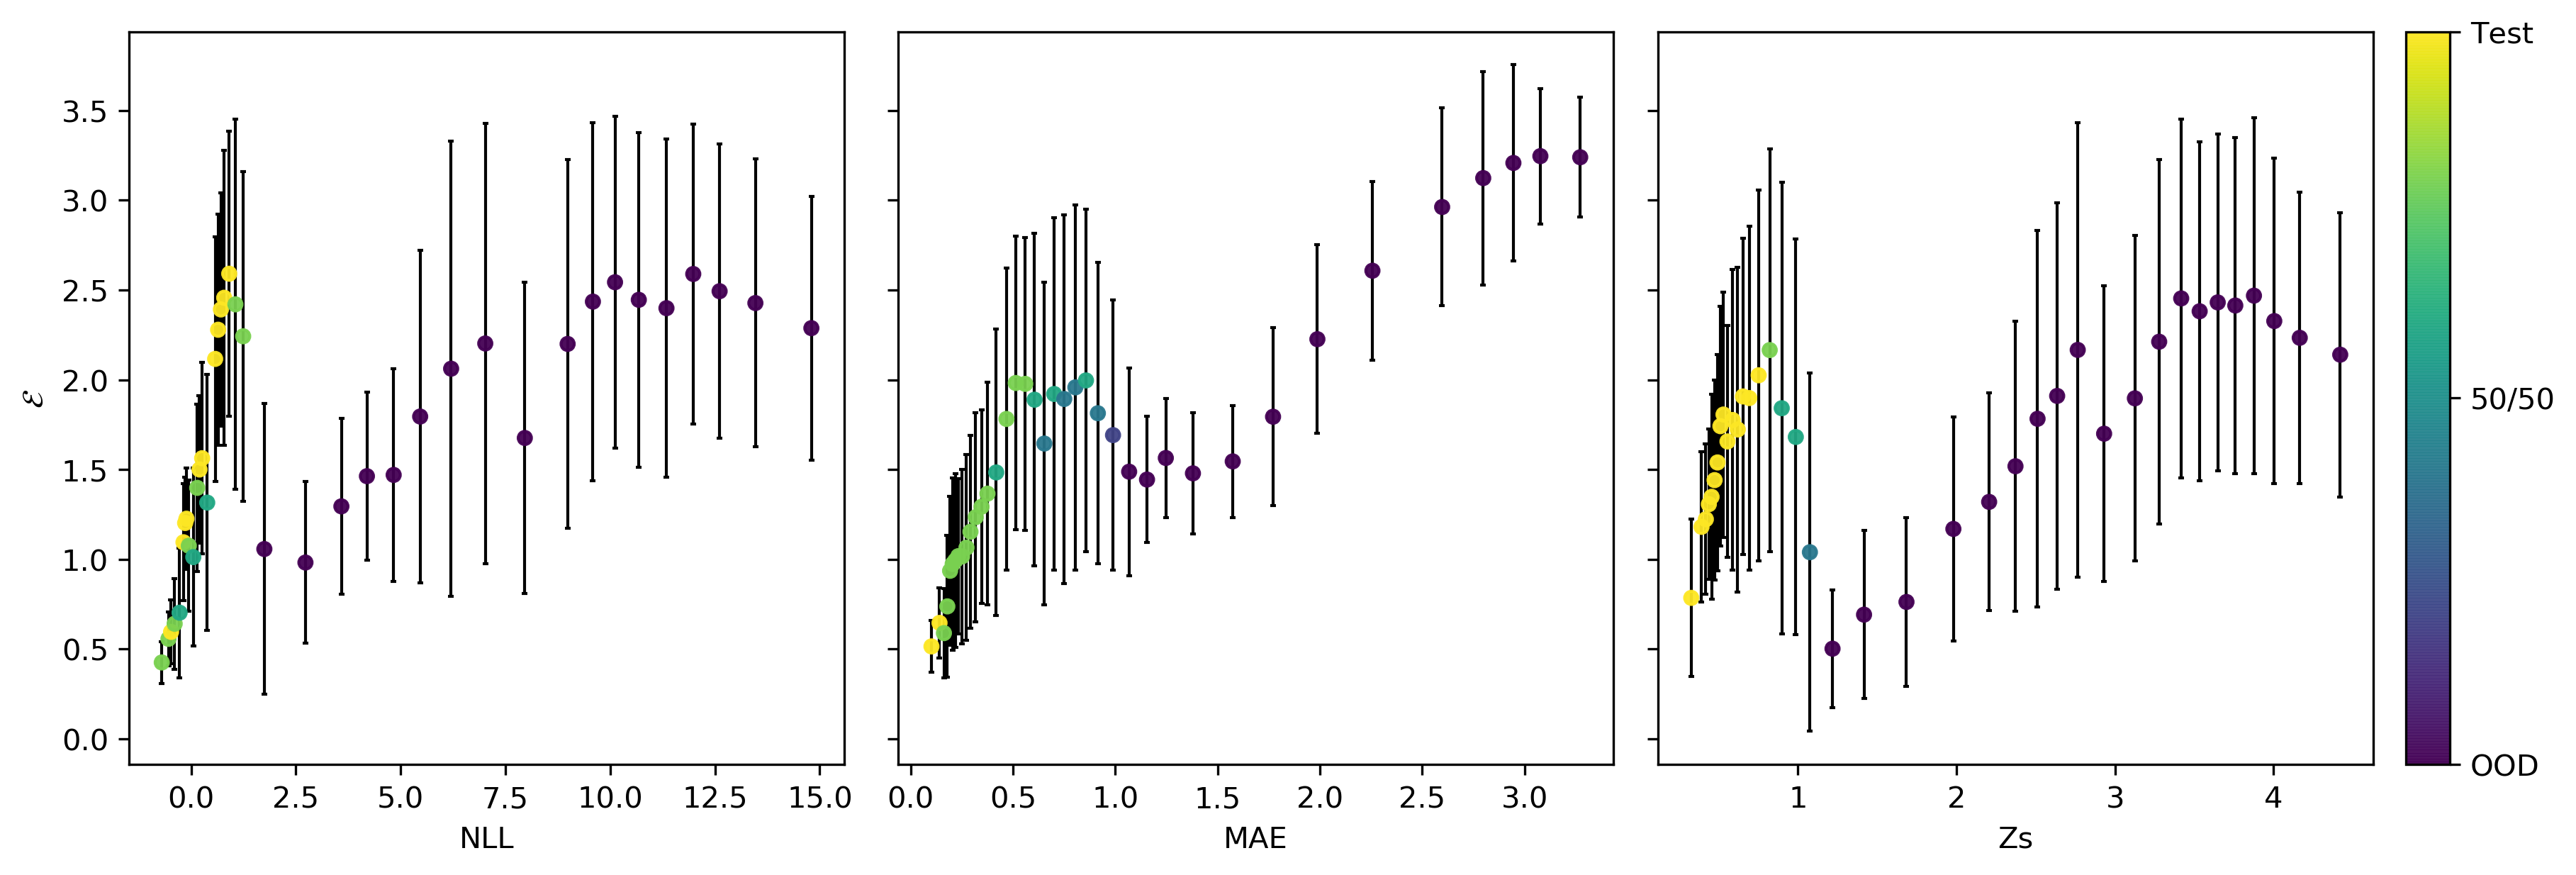
\includegraphics[width=\textwidth]{Experiments/figs/binned/bb2_dropout_epistemic.png}
        \caption{Binned diagonal plots for the epistemic uncertainty.}
    \end{subfigure}
    
    \begin{subfigure}[b]{\textwidth}
        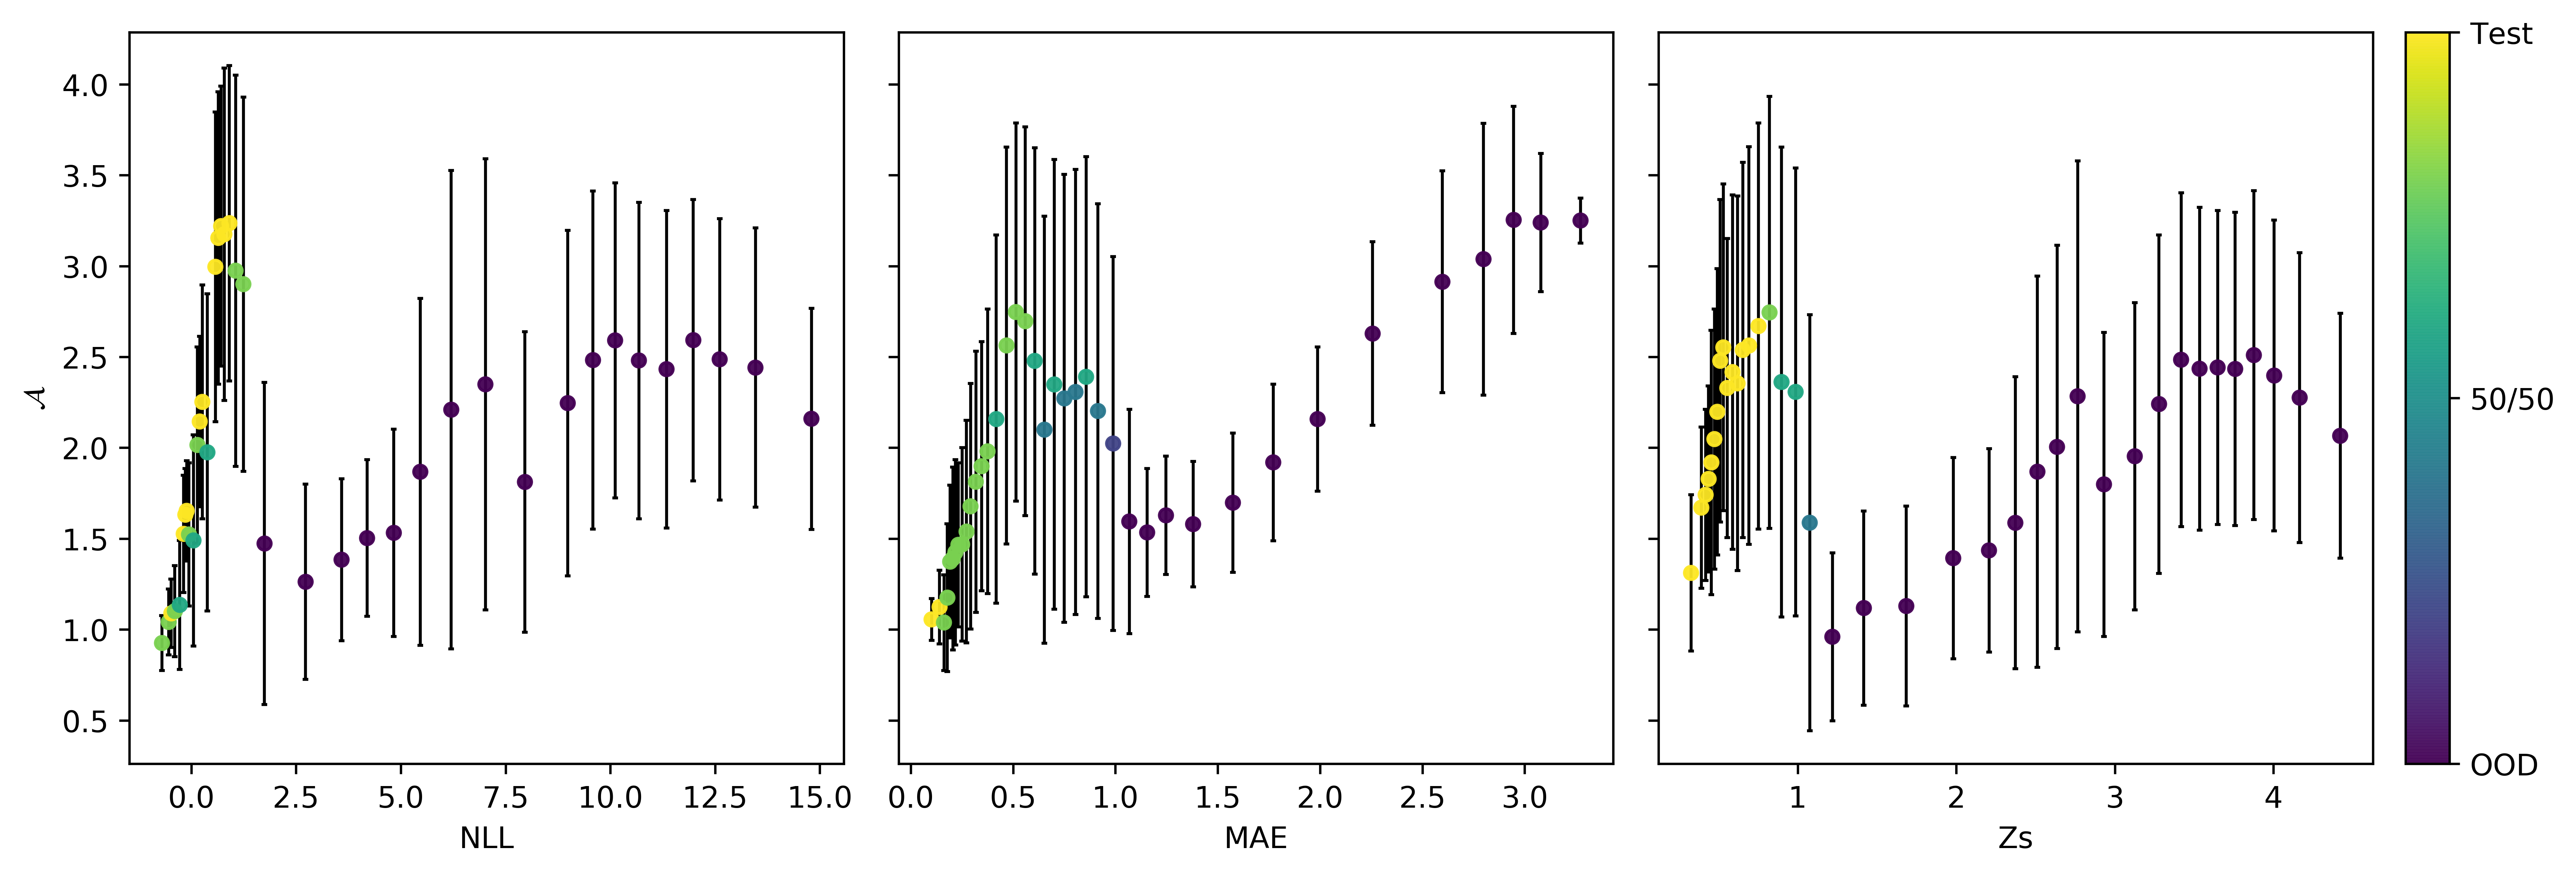
\includegraphics[width=\textwidth]{Experiments/figs/binned/bb2_dropout_aleatoric.png}
        \caption{Binned diagonal plots for the aleatoric uncertainty.}
  \end{subfigure}
    \caption[Blackbird(2) error-uncertainty diagonal plots for MC dropout]{Blackbird(2) error-uncertainty diagonal plots for MC dropout. For plot description see \cref{sec:crnn_analysis}}
    \label{fig:bb2_dropout_uncertainty_corr}
\end{figure}

\Cref{fig:bb2_dropout_uncertainty_corr} shows the binned diagonal plots for errors versus uncertainties. For both uncertainties, we see the familiar pattern of the uncertainty correlating with the error in the beginning then \emph{resetting} and correlated separately with the tail. The plots also give visual testimony to the notion that MC dropout's epistemic uncertainty overlaps highly with the aleatoric uncertainty in terms of information about the errors. Comparing the plots here with the ones for C-RNN(\cref{fig:bb2_uncertainty_corr}), we can see that C-RNN's epistemic uncertainty gives information that MC dropout does not capture. Not just for better separating in/out-of-distribution data, but also  a stronger correlation with the error for the OOD inputs. We will distill the key findings for Blackbird(2) in the next section. 

\clearpage
\subsection{Key findings}

In general, the findings of this section go along the same lines of the findings in \cref{sec:revs_results}. We find that 

\begin{itemize}
    \item The epistemic uncertainty from C-RNN is useful in separating the in/out-of-distribution inputs.
    \item The epistemic uncertainty from MC dropout is of no use in separating the in/out-of-distribution inputs.
    \item For C-RNN the epistemic and aleatoric uncertainties are moderately correlated, but the epistemic uncertainty provides more information. 
    \item For MC dropout the aleatoric and epistemic uncertainties are strongly correlated and seem to provide the same information. 
\end{itemize}{}


In \cref{tbl:bb2_comparison} we have a summary of the key metrics for comparison of C-RNN and MC dropout. The table supports our key findings, we can see that C-RNN gets an AUROC of 0.8, whereas MC dropout gets an AUROC of 0.48, showing that C-RNN has some success in separating in/out-of-distribution inputs and MC dropout is performing as well as random guessing. MC dropout has high correlation between epistemic uncertainty over each split individually with 0.84 and 0.91 Pearson coefficient for the test and OOD splits respectively, but an 0.69 Pearson coefficient for the combined splits, whereas C-RNN has a Pearson coefficient of 0.9 over the combined splits.  

\begin{table*}[h]
\centering
    \begin{tabular}{l l c c c c c}  
        \toprule
        Model & split & MAE & NLL & $\rho$(MAE vs $\mathcal{E}$) &
        $\rho$(Z-score vs $\mathcal{E}$) & AUROC($\mathcal{E}$)\\
        \midrule
        \multirow{3}{*}{C-RNN} 
            & Test     & 0.27 & 0.22 & 0.92 & 0.48 & - \\  
            & OOD      & 1.12 & 11.2 & 0.87 & 0.83 & -\\  
            & Test+OOD & 0.7  & 5.7  & 0.9  & 0.83 & 0.8\\ 

        \midrule
        \multirow{3}{*}{MC dropout} 
            & Test     & 0.27 & 0.22 & 0.84  & 0.43 & - \\  
            & OOD      & 1.1 & 7.3   & 0.91  & 0.54 & -\\  
            & Test+OOD & 0.69 & 3.7  & 0.69  & 0.31 & 0.48\\ 

        \toprule
    \end{tabular}
    \caption{Blackbird(2) key results for comparison of C-RNN and MC dropout.}
    \label{tbl:bb2_comparison}
\end{table*}

So far, we have conducted experiments over two datasets and three different settings overall. We saw numerous patterns persist. In the next section, we will distill the patterns we found in all our experiments.



\clearpage
\section{Summary of findings}

The results of the last three sections have shown some patterns. In this section, we will look at all our experiments together, present a compact version of the key results and distill the findings that come out.

Our focus will be on the comparison between C-RNN and MC dropout, particularly in terms of quality and behavior of epistemic uncertainty. 

Before we get to our substantive issue, we start with two general observation about the aleatoric uncertainty. In all of our experiments the aleatoric uncertainty performs close to random in terms of separating the in/out-of-distribution inputs. The highest AUROC we have seen using the aleatoric uncertainty is 0.57, which is only slightly better than expected random behavior. This holds for both C-RNN and MC dropout. The aleatoric uncertainty still provides useful information about the error as we have seen from the results. However we will be focusing on the epistemic uncertainty for our comparison between C-RNN and MC dropout, since this is where the the two models differ significantly and this is the uncertainty we need most when OOD samples are present.    

% This brings us to our second point regarding the aleatoric uncertainty, which is that both models we used in our experiments estimate it in the same. Granted the different training induced by dropout may lead to models with different behavior when predicting the aleatoric uncertainty. However, we have just mentioned that for both models, it fails to separate the test and OOD splits. Moreover, \cref{tbl} shows the Pearson correlation between the aleatoric uncertainty and the MAE for both models mover all datasets side by side. 


\subsubsection{C-RNN vs. MC dropout}

We start this comparison by collecting the MAE and NLL for both models over all datasets in \cref{tbl:comparison}. In general the performance is similar with each model providing better numbers in some settings. We can see that MC dropout get better NLL for the OOD splits on Revs and Blackbird(2), despite not having lower MAE. On the other hand, we can see that C-RNN gets better performance on the Revs test split, with an MAE of 0.55 to MC dropout's 1.26. Beyond that basic performance seems to be similar. 

% \begin{table*}[htbp]
% \centering
%     \begin{tabular}{l l c c c c c c}  
%         \toprule
%         Model & split & \multicolumn{3}{c}{MAE} & \multicolumn{3}{c}{NLL}\\
%         - & - & Revs & Blackbird(1) & Blackbird(2) & Revs & Blackbird(1) & Blackbird(2) \\
%         \midrule
%         \multirow{3}{*}{C-RNN} 
%             & Test     & 0.55 & 0.3 & 0.27  & 0.44   & 0.3  & 0.22 \\  
%             & OOD      & 2.6 & 0.27 & 1.12  & 17.8   & 0.13 & 11.2\\  
%             & Test+OOD & 1.6 & 0.28 & 0.7   & 9.2    & 0.21 & 5.7\\ 

%         \midrule
%         \multirow{3}{*}{MC dropout} 
%             & Test     & 1.26 & 0.26 & 0.27  & 1.14 & 0.2   & 0.22 \\  
%             & OOD      & 2.55 & 0.28 & 1.1  & 1.62  & 0.23  & 7.3 \\  
%             & Test+OOD & 1.8  & 0.27 & 0.69  & 1.38 & 0.21  & 3.7\\ 
        
%         \toprule
%     \end{tabular}
%     \caption{Performance metrics.}
%     \label{tbl:comparison}
% \end{table*}

\begin{table*}[htbp]
\centering
    \begin{tabular}{l l c c c c c c}  
        \toprule
        Model & split & \multicolumn{2}{c}{Revs} & \multicolumn{2}{c}{Blackbird(1)} & \multicolumn{2}{c}{Blackbird(2)}\\
        - & - & MAE & NLL & MAE & NLL & MAE & NLL \\
        \midrule
        \multirow{3}{*}{C-RNN} 
            & Test     & 0.55 & 0.44 & 0.3  & 0.3   & 0.27 & 0.22 \\  
            & OOD      & 2.6  & 17.8 & 0.27 & 0.13  & 1.12 & 11.2\\  
            & Test+OOD & 1.6  & 9.2  & 0.28 & 0.21  & 0.7  & 5.7\\ 

        \midrule
        \multirow{3}{*}{MC dropout} 
            & Test     & 1.26 & 1.14 & 0.26  & 0.2   & 0.27 & 0.22 \\  
            & OOD      & 2.55 & 1.62 & 0.28  & 0.23  & 1.1  &  7.3 \\  
            & Test+OOD & 1.8  & 0.26 & 0.27  & 0.21  & 0.69 & 3.7\\ 
        
        \toprule
    \end{tabular}
    \caption{Predictive performance comparison.}
    \label{tbl:comparison}
\end{table*}


The main difference between C-RNN and MC dropout is the estimation of the epistemic uncertainty. We have argued in \cref{ch:background} that the standard Bayesian framework that MC dropout is unreliable for estimating uncertainty when OOD data can be present at inference time. The results of our experiments have supported this claim. In \cref{tbl:epistemic_comparison} we compare the performance of the epistemic uncertainty for MC dropout and C-RNN in terms of correlation with the errors and discrimination between in/out-of-distribution inputs. 

\begin{table*}[htbp]
\centering
\begin{adjustbox}{max width=\textwidth}
    \begin{tabular}{l l c c c c c c}  
        \toprule
        Model & split & \multicolumn{2}{c}{Revs} & \multicolumn{2}{c}{Blackbird(1)} & \multicolumn{2}{c}{Blackbird(2)}\\
        - & - & $\rho$(MAE vs $\mathcal{E}$) & AUROC &
        $\rho$(MAE vs $\mathcal{E}$) & AUROC & $\rho$(MAE vs $\mathcal{E}$)  & AUROC \\
        \midrule
        \multirow{3}{*}{C-RNN} 
            & Test     & 0.32 & -    & 0.88 & -    & 0.92 & -   \\  
            & OOD      & 0.57 & -    & 0.9  & -    & 0.87 & -   \\  
            & Test+OOD & 0.85 & 0.97 & 0.88 & 0.46 & 0.9  & 0.8 \\ 

        \midrule
        \multirow{3}{*}{MC dropout} 
            & Test     & 0.36 & -    & 0.76  & -    & 0.84 & -  \\  
            & OOD      & 0.32 & -    & 0.77  & -    & 0.91  &  -  \\  
            & Test+OOD & 0.41 & 0.64 & 0.76  & 0.46 & 0.69 & 0.48 \\ 
        
        \toprule
    \end{tabular}
\end{adjustbox}
    \caption[Epistemic uncertainty comparison]{Epistemic uncertainty comparison. We show the Pearson correlation with the MAE, and the AUROC.}
    \label{tbl:epistemic_comparison}
\end{table*}

Recall that the AUROC measure here represents the probability that a randomly chosen in-distribution input is assigned lower epistemic uncertainty than a random OOD input. We can see that C-RNN significantly out-preforms MC dropout on both the Revs and Blackbird(2) experiments. When the errors on the OOD data is significantly higher than on test data, this is a desirable property, and this is in fact the case for Revs and Blackbird(2). However we have seen on Blackbird(1) that we can have OOD inputs where the model can generalize well, and ideally we do not want high uncertainty for such inputs. We can see from \cref{tbl:epistemic_comparison} that C-RNN does not give higher uncertainty to OOD data in Blackbird(1), with an AUROC of 0.46. 

\begin{figure}[htbp]
  \centering
    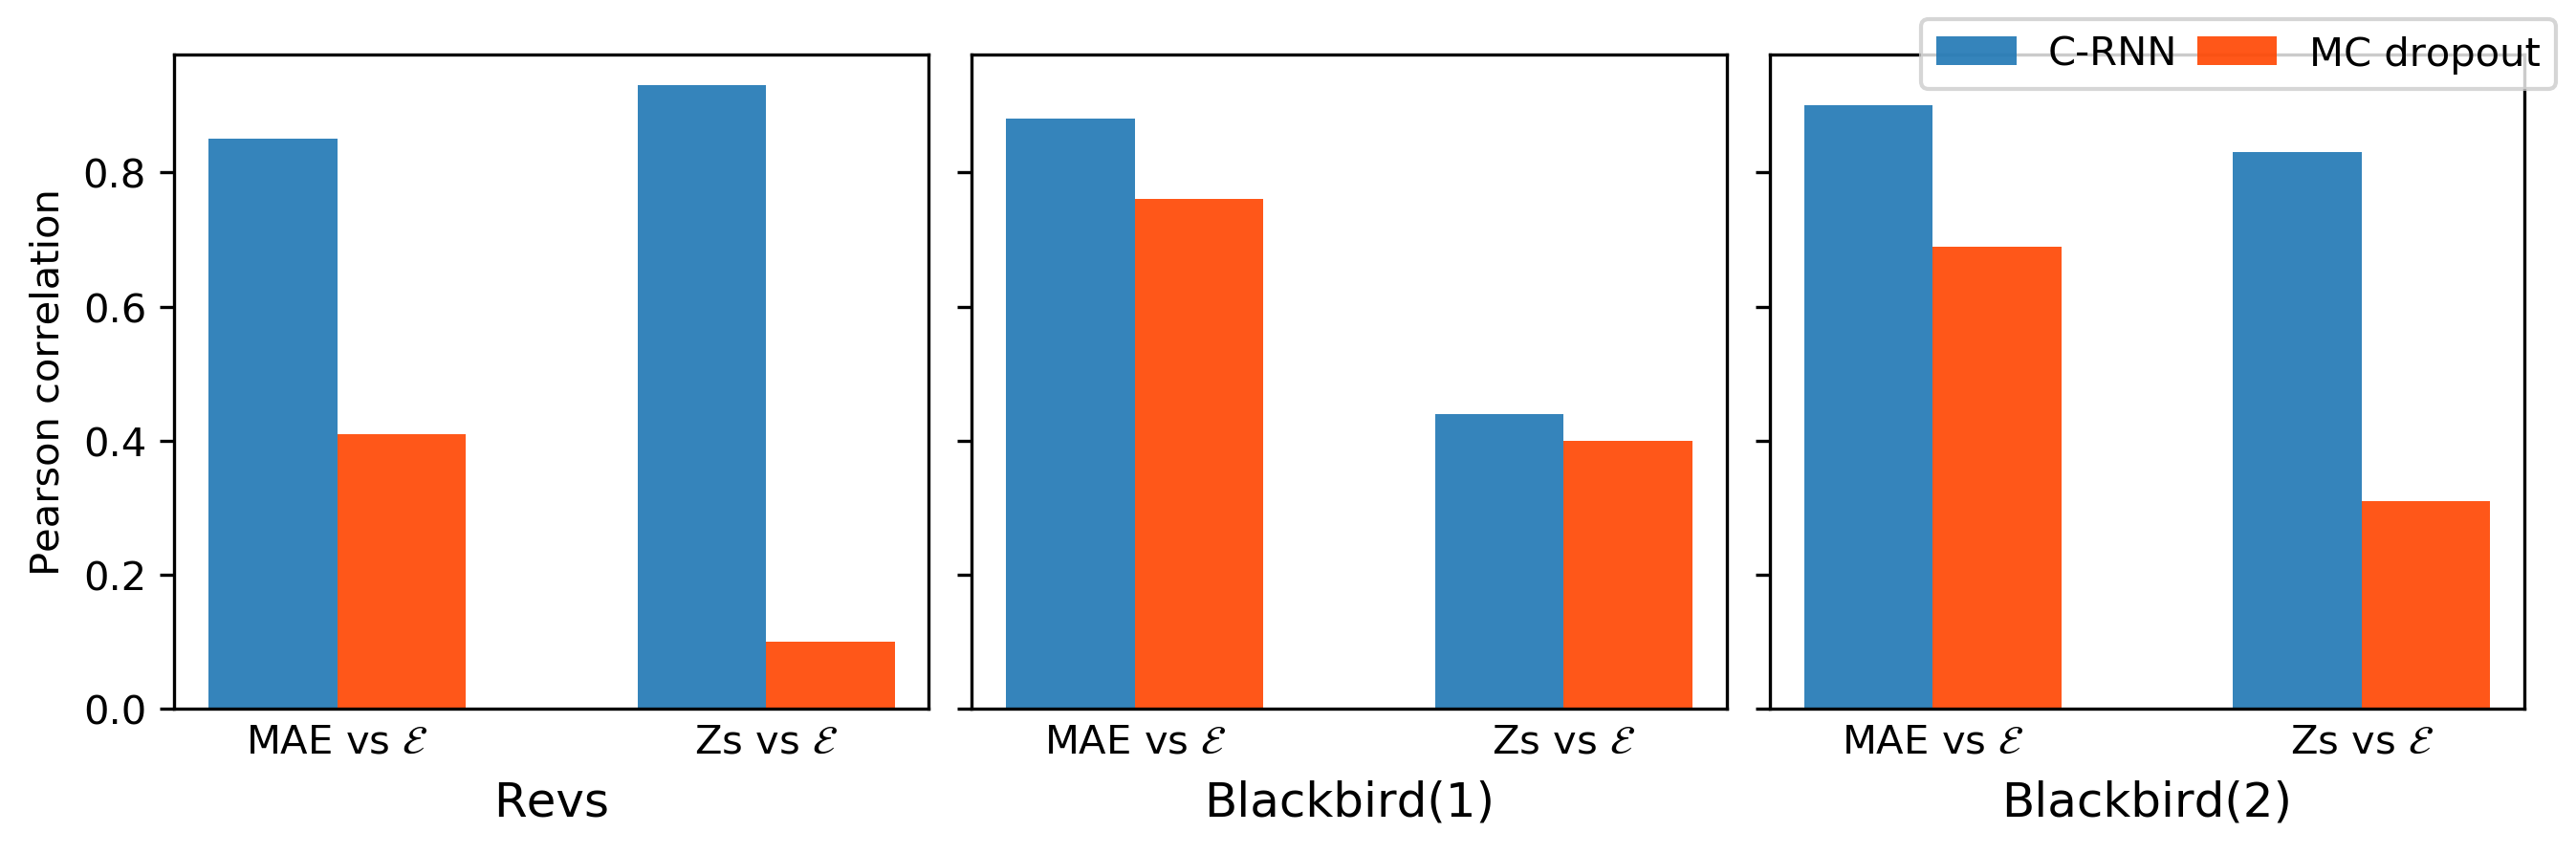
\includegraphics[width=\textwidth]{Experiments/figs/correlation_comparison.png}

    \caption[Comparison of error-uncertainty correlations for C-RNN and MC dropout]{Bar chart for comparing the correlations, between the epistemic uncertainty and the error scores(MAE, Z-score) over the test+OOD split, for C-RNN and MC dropout}
    \label{fig:epistmic_comparison}
\end{figure}


In terms of correlation between the errors and the uncertainties, we can see, from \cref{tbl:epistemic_comparison} and \cref{fig:epistmic_comparison}, that C-RNN consistently outperforms MC dropout when looking at the combined split. Of course, the combined split represents the type of real world use cases we are interested in. However, the somewhat more impressive finding, is that over the test split alone C-RNN still consistently out-preforms MC dropout, albeit by a smaller margin.  

To conclude, we have shown over three different sets of experiments that C-RNN can give reliable uncertainty estimates in settings where data comes from a mixture on in and out-of-distribution, which is our target use case. Moreover, even in the absence of OOD samples, or when the model can generalize well to OOD samples, C-RNN's epistemic uncertainty remains a valid signal for uncertainty, and performs as well or better than MC dropout's epistemic uncertainty. 

% In the next chapter, we will conduct a literature review  




\end{document}  

